\documentclass[
    %iai, % Saisir le nom de l'institut rattaché
    mi, % Saisir le nom de l'orientation
    %confidential, % Décommentez si le travail est confidentiel
,table]{heig-tb}

\usepackage[nooldvoltagedirection,european,americaninductors]{circuitikz}
\usepackage[T1]{fontenc}
\usepackage{xcolor}
\usepackage{hyperref}
%\usepackage{biblatex}

\signature{mbernasconi.svg} % Remplacer par votre propre signature vectorielle.

\makenomenclature
\makenoidxglossaries
\makeindex

\addbibresource{bibliography.bib}

\input{nomenclature}
\input{acronyms}
\input{glossary}
% Auteur du document (étudiant-e) en projet de Bachelor
\author{Antoine Oberson}

% Activer l'option pour l'accord du féminin dans le texte
%\genre{female}

% Titre de votre travail de Bachelor
\title{Rapport de travail de Bachelor}

% Le sous titre est optionnel
\subtitle{Générateur de turbulence optique pour le test de systèmes de propagation de faisceau à travers l'atmosphère terrestre}


% Nom du professeur responsable
\teacher {Prof. Jolissaint Laurent(HEIG-VD)}

% Mettre à jour avec la date de rendu du travail
\date{\today}

% Numéro de TB
\thesis{7212}



\surroundwithmdframed{minted}

%% Début du document
\begin{document}
\selectlanguage{french}
\maketitle
\frontmatter
\clearemptydoublepage

%% Requis par les dispositions générales des travaux de Bachelor
\preamble
\authentification

%% Résumé / Résumé publiable / Version abrégée
\begin{abstract}
    % Francais
%\lipsum[1]

\asterism

% English
\lipsum[3]

\end{abstract}

%% Sommaire et tables
\clearemptydoublepage
{
    \tableofcontents
    \let\cleardoublepage\clearpage
    \listoffigures
    \let\cleardoublepage\clearpage
    \listoftables
    \let\cleardoublepage\clearpage
    \listoflistings
}

\printnomenclature
\clearemptydoublepage
\pagenumbering{arabic}

\hypersetup{
    colorlinks=true,
    linkcolor=blue,
    filecolor=magenta,      
    urlcolor=cyan,
    pdftitle={Overleaf Example},
    pdfpagemode=FullScreen,
}

%% Contenu
\mainmatter
\chapter{Introduction}
%L'introduction est une section requise dans un rapport technique. Introduisez votre travail, l'idée de départ et les objectifs attendus. Un lecteur qui découvrirait votre projet au travers de cette introduction devrait ainsi être capable d'en comprendre le cadre, l'idée générale et les aboutissants du projet.

En 2014, le laboratoire d'optique (Optolab.iai) de l'HEIG-VD a produit le design optique et les instruments de 1ère génération du \href{https://atasam.atauni.edu.tr/}{DAG (Dogu Anadolu Gözlemevi, Eastern Anatolia Observatory)}\footnotemark
un téléscope optique et infrarouge proche de 4m de diamètre situé en Turquie à 3000m d'altitude dans les montagnes Palandöken proche de la ville d'Erzurum en Anatolie de l'est.Plus précisémment aux collines de Karakaya, cette région fut sélectionnée pour sa faible humidité, le vent y est faible et sa direction est stable
,le nombre de jours et nuits clairs, une ville est à proximité mais elle n'est pas visible depuis la localisation du DAG, il y a donc peu de pollution lumineuse, ces caractéristiques atmosphériques et structurelles en font donc un endroit propice à l'installation de plusieur grand téléscope permettant entre autre l'observation
dans l'infrarouge proche (ce qui est possible dans peu d'endroits au monde).

Malheureusement, même avec les conditions atmosphériques et géographiques les plus parfaites, le téléscope fait toujours face à un grand ennemi : \textbf{les turbulences}.
Le travail actuel d'Optolab est donc de développer un système d'optique adaptative ayant pour but de contrer les turbulences optiques produites par l'atmosphère. Ce système
d'optique adaptative a besoin d'être testé à l'aide d'écrans circulaires permettant de simuler des turbulances optiques.

Dans le cadre de ce projet de Bachelor, il convient donc de reprendre le travail réalisé dans un projet de Master précédent de l'HES-SO, ce dernier consistait en une boîte permettant de projeter un gas d'acrylique transparente sur une plaque de plastique, elle aussi, transparente. La turbulence du nuage de gas
d'acrylique immortalise sur la plaque en plastique une différence de chemin optique similaire à la distribution de la turbulence optique.

Le but de ce travail de Bachelor est donc de comprendre le fonctionnement de la machine de projection pour en suite l'améliorer afin de produire in-situ des écrans de phase calibrés.
\footnotetext{\url{https://atasam.atauni.edu.tr/}}

\newpage


\section{Contexte}
Cette section \underline{n'est pas obligatoire}, mais elle est souvent présente dans un rapport technique pour compléter l'introduction et définir le contexte du travail \cad le cadre formel dans lequel le travail est mené.




\chapter{Améliorations}
\section{Porte}
Sur l'image ci-dessous, la porte dans son état original :
\begin{figure}[H]
    \centering
    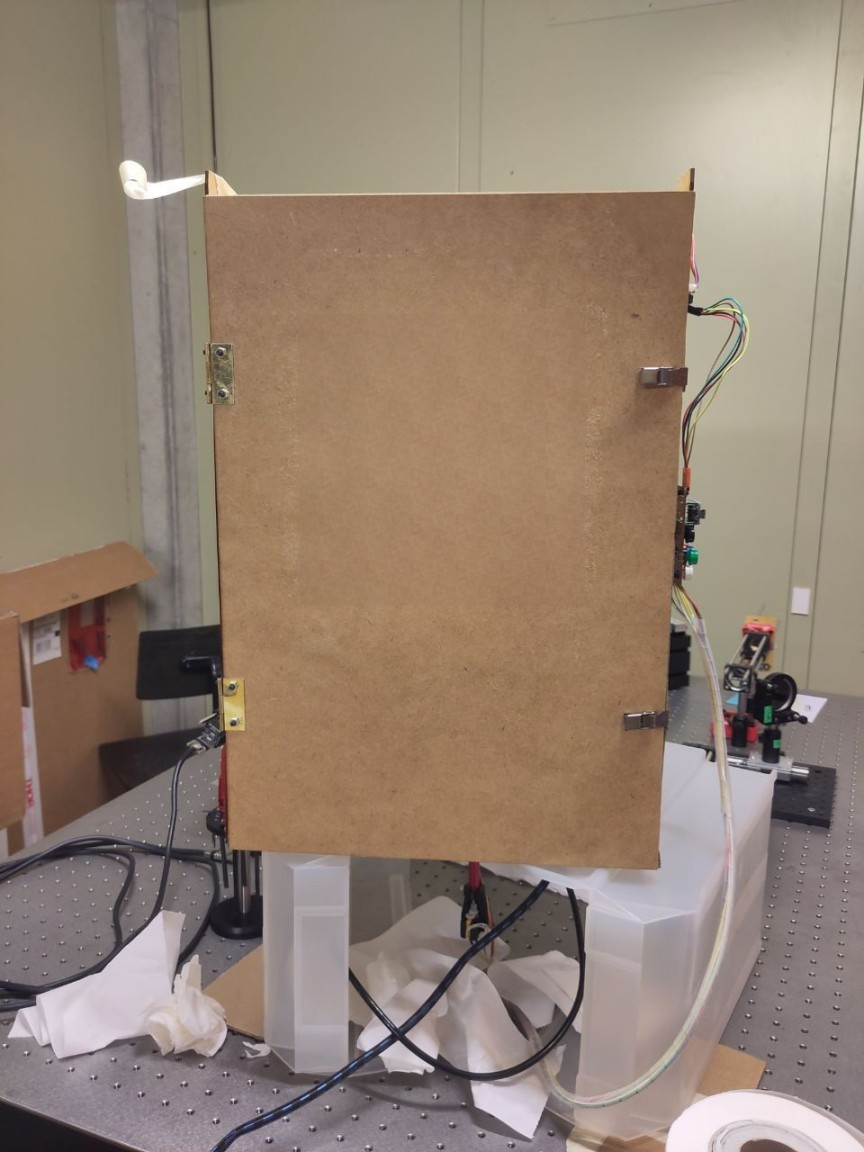
\includegraphics[width=0.5\textwidth]{assets/figures/ameliorations/porte_sans_fenetre.png}
    \caption{Photo de la porte avant modification}\label{photo porte}
\end{figure}

\newpage
Après une découpe dans le panneau de la porte, et le design de pièces de fixations et d'un chablon de perçage,
la porte est désormais équipée d'une fenetre:
\begin{figure}[H]
    \centering
    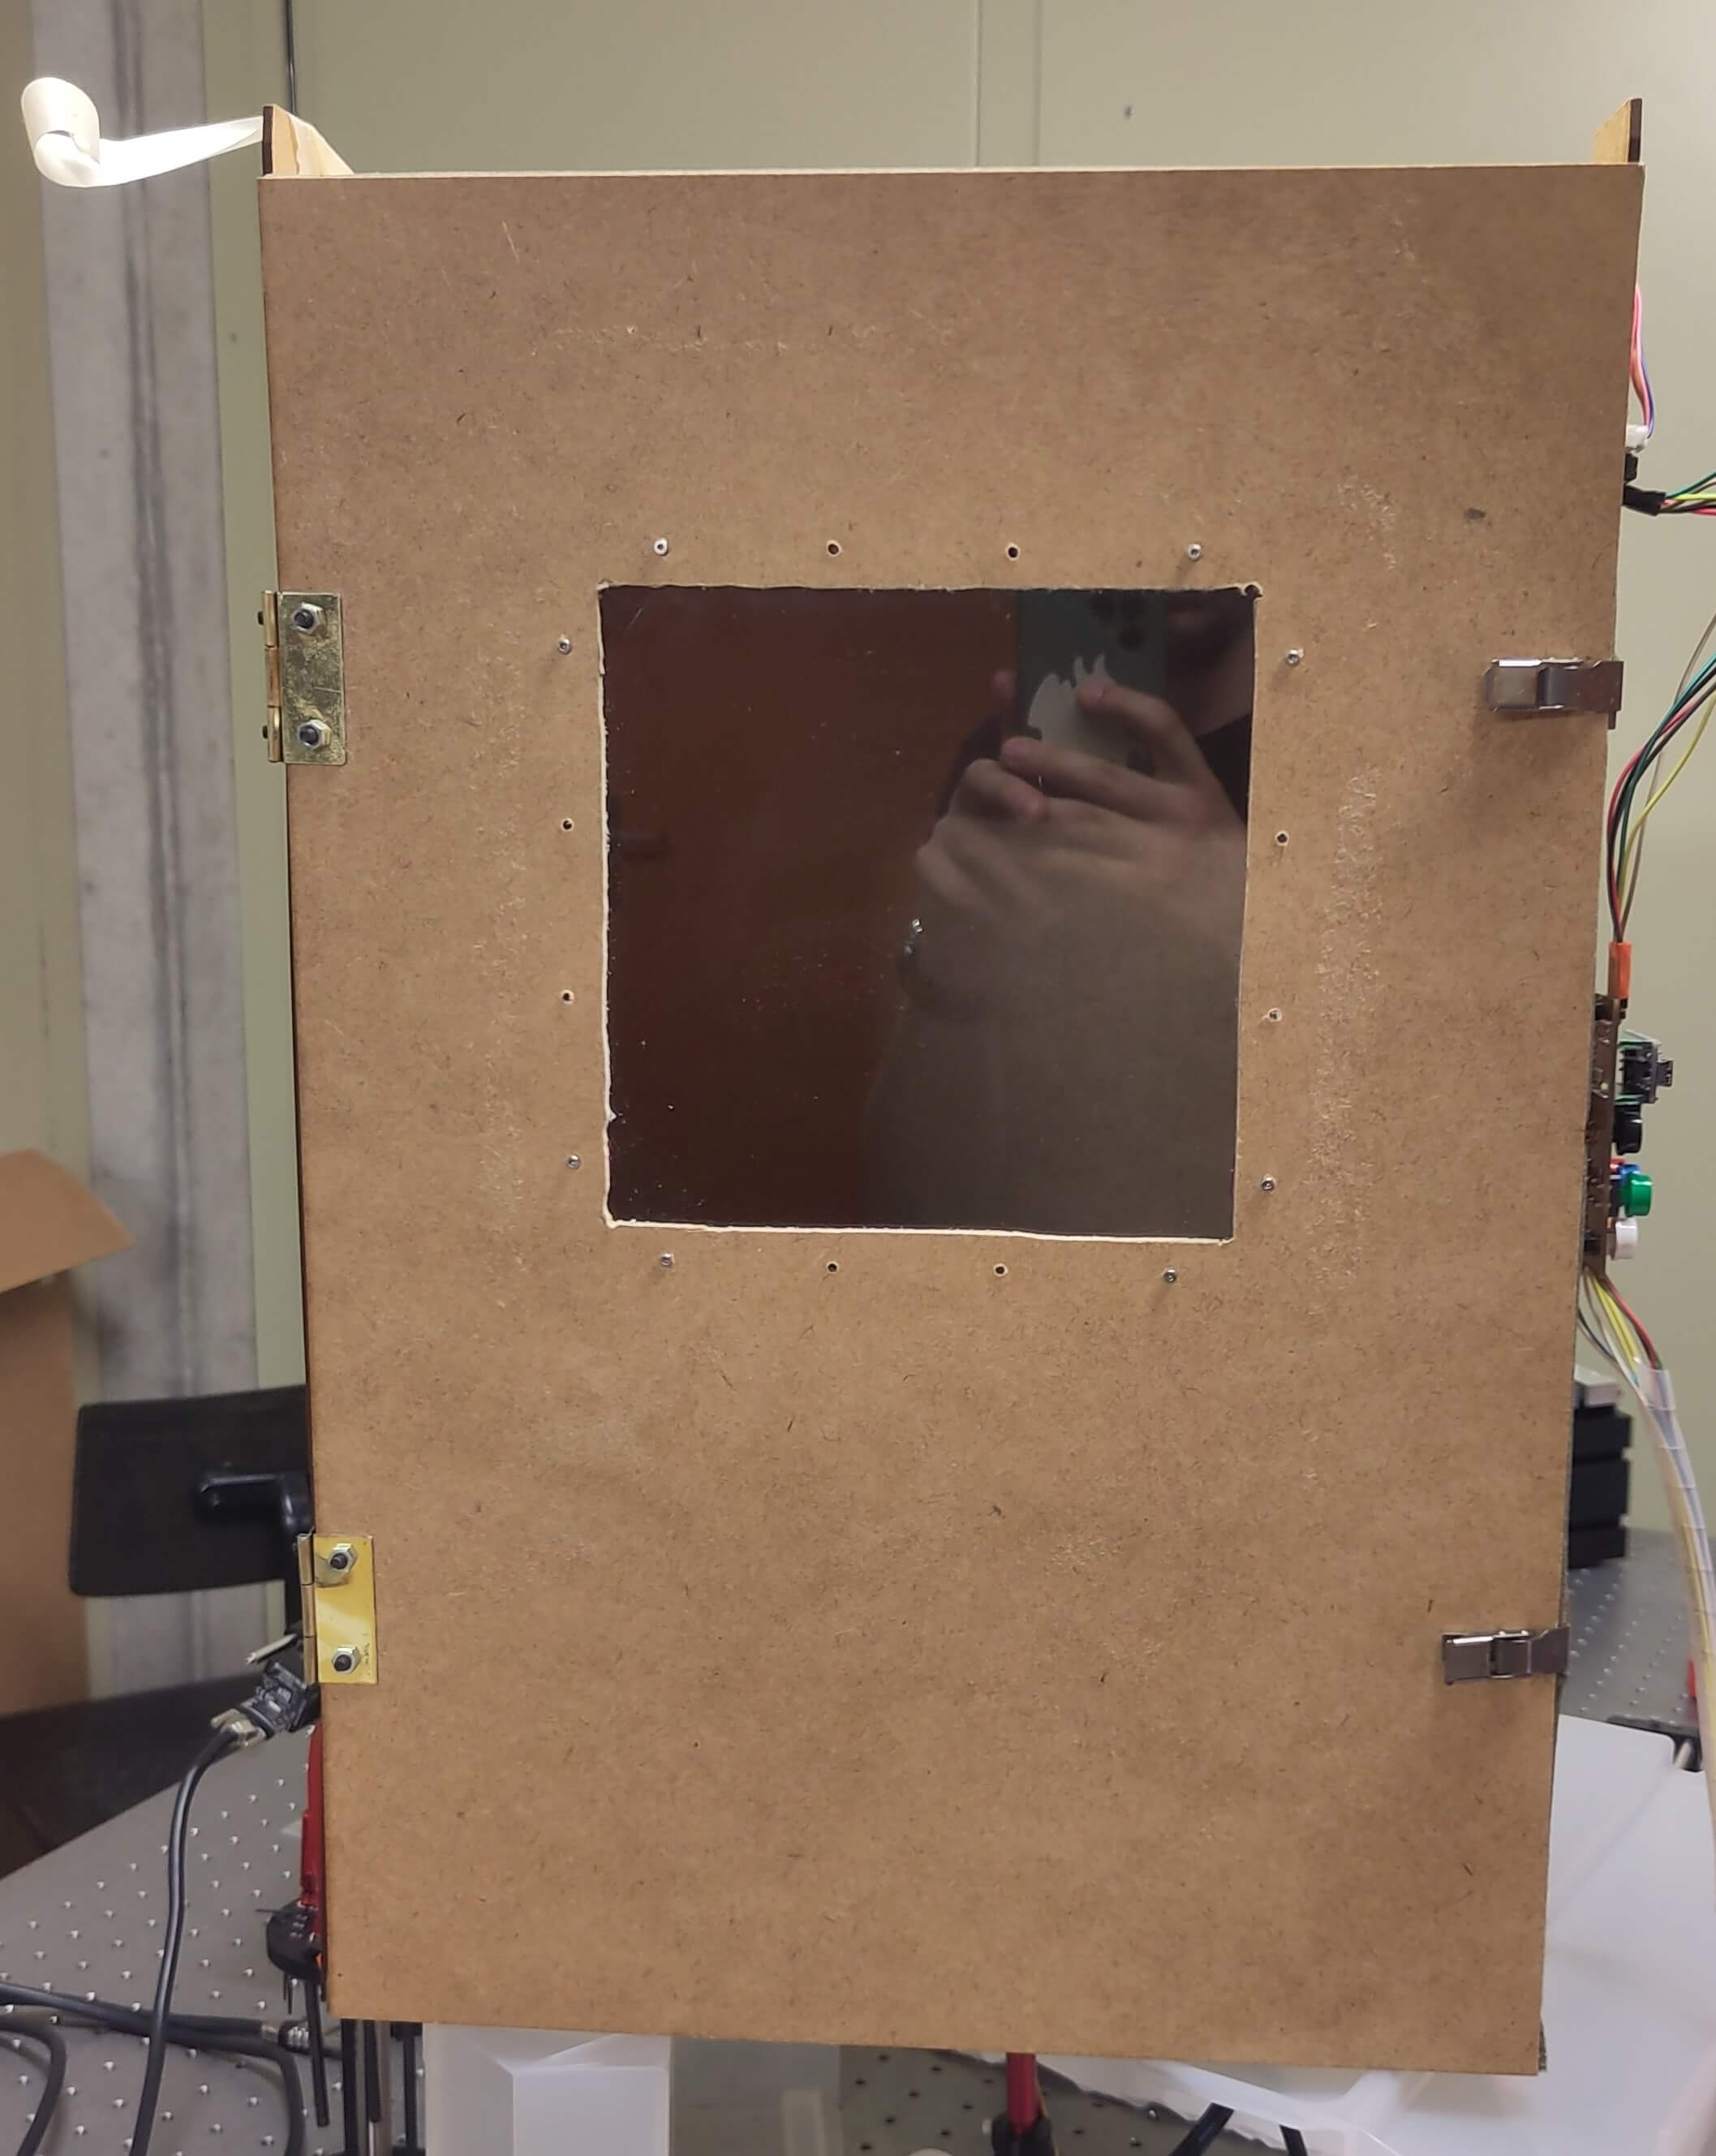
\includegraphics[width=0.5\textwidth]{assets/figures/ameliorations/porte_avec_fenetre.jpg}
    \caption{Photo de la porte après modification}\label{photo porte fenetre}
\end{figure}

La vitre est fixée à l'aide de petites broches vissées dans le bois :
\begin{figure}[H]
    \centering
    \begin{subfigure}{.5\textwidth}
        \centering
        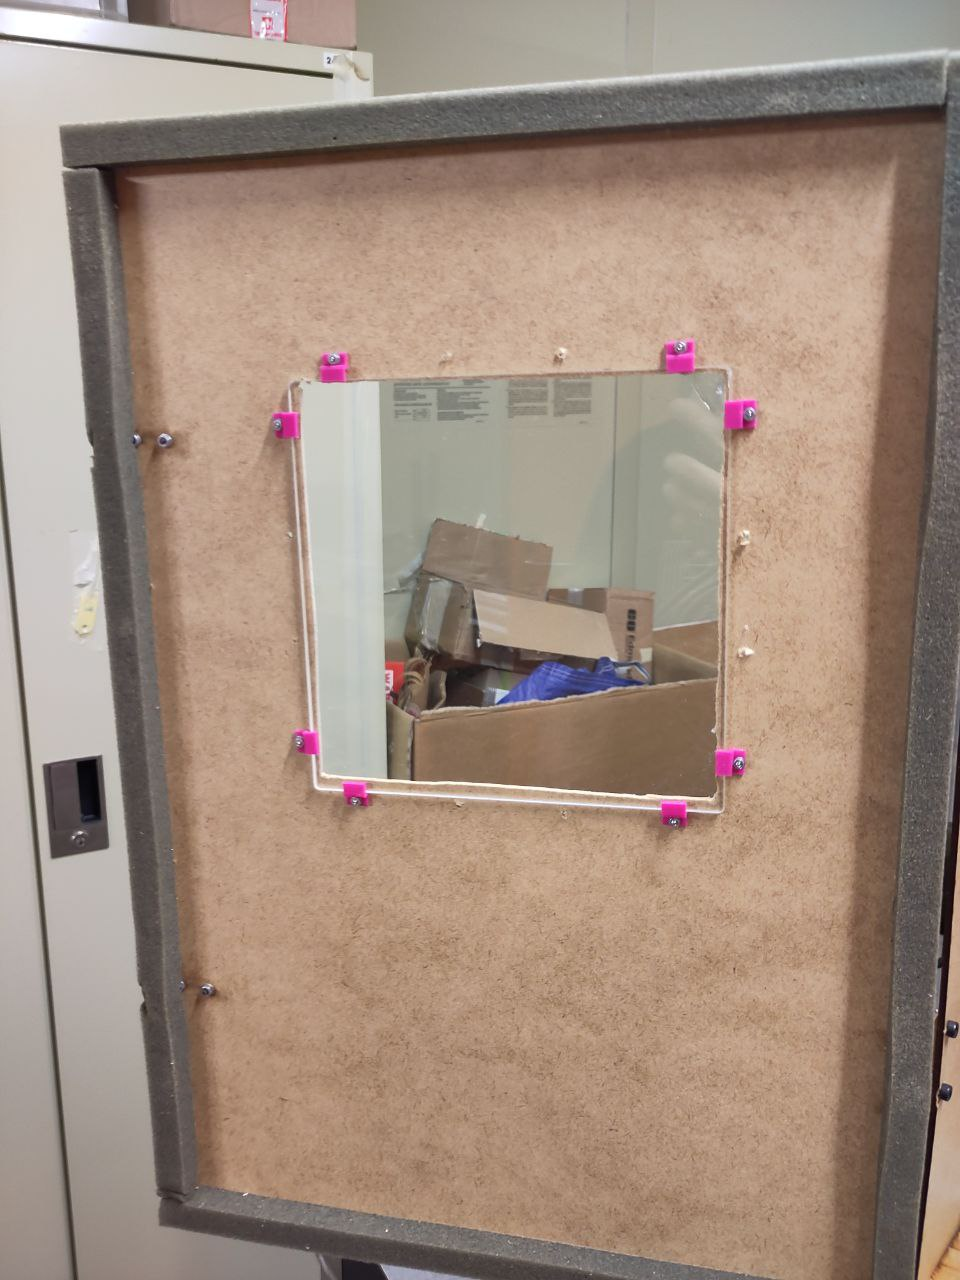
\includegraphics[width=1\linewidth,trim = 250 420 180 300, clip]{assets/figures/ameliorations/fixation_vitre.jpg}
        \caption{Vitre fixée}
        \label{fig:vitre_fixee}
    \end{subfigure}%
    \begin{subfigure}{.5\textwidth}
        \centering
        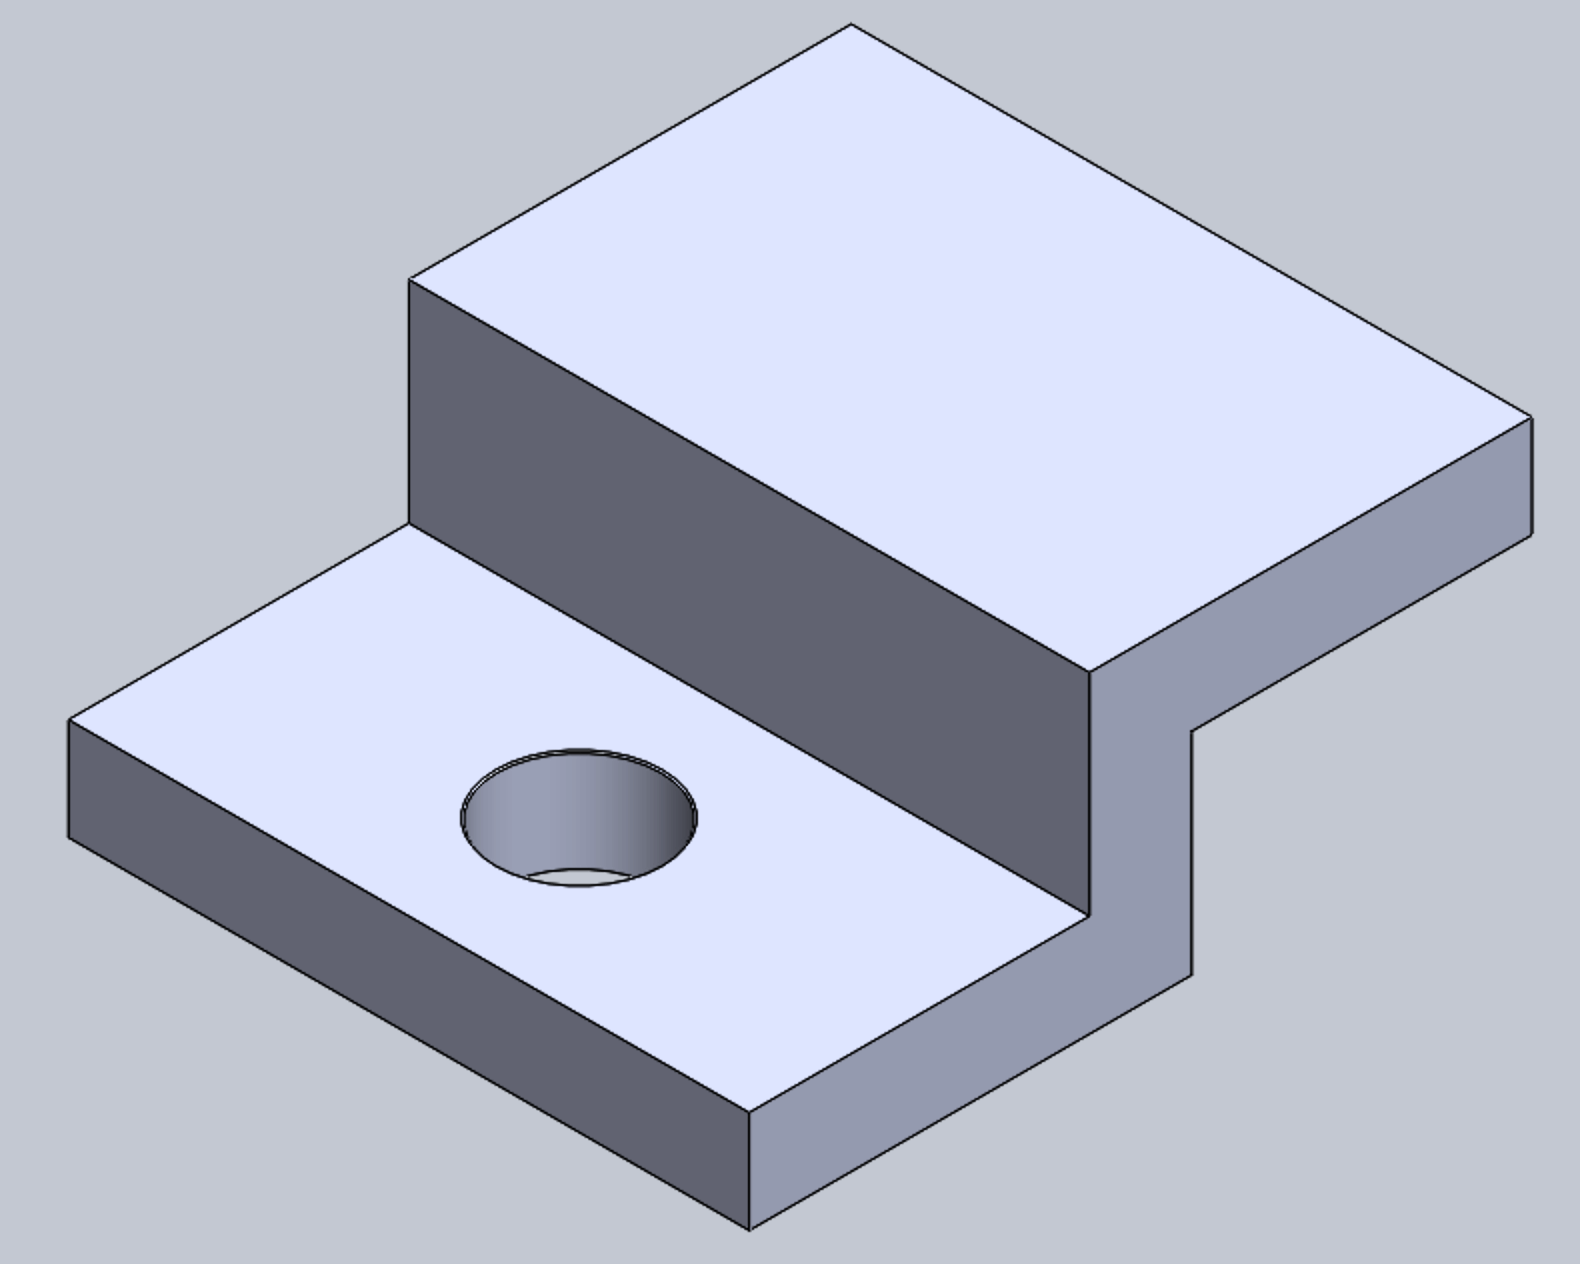
\includegraphics[width=.75\linewidth]{assets/figures/ameliorations/broche_vitre.png}
        \caption{Broche de fixation de la vitre}
        \label{fig:broche_fixation_vitre}
    \end{subfigure}
    \caption[Illustration de la fixation de la vitre]{Illustration de la fixation de la vitre}
    \label{fig:illu_vitre_porte}
\end{figure}
Le chablon pour les trous est trouvable dans l'\autoref{chablon_trous_vitre}.
\newpage
\section{Mesures}
\subsection{Problématique et situation d'origine}
Le procédé de mesure d'origine est sommaire et nécessite beaucoup de temps, en effet il convient de:
\begin{enumerate}
    \item Placer le disque dans le faisceau :
          \begin{figure}[H]
              \centering
              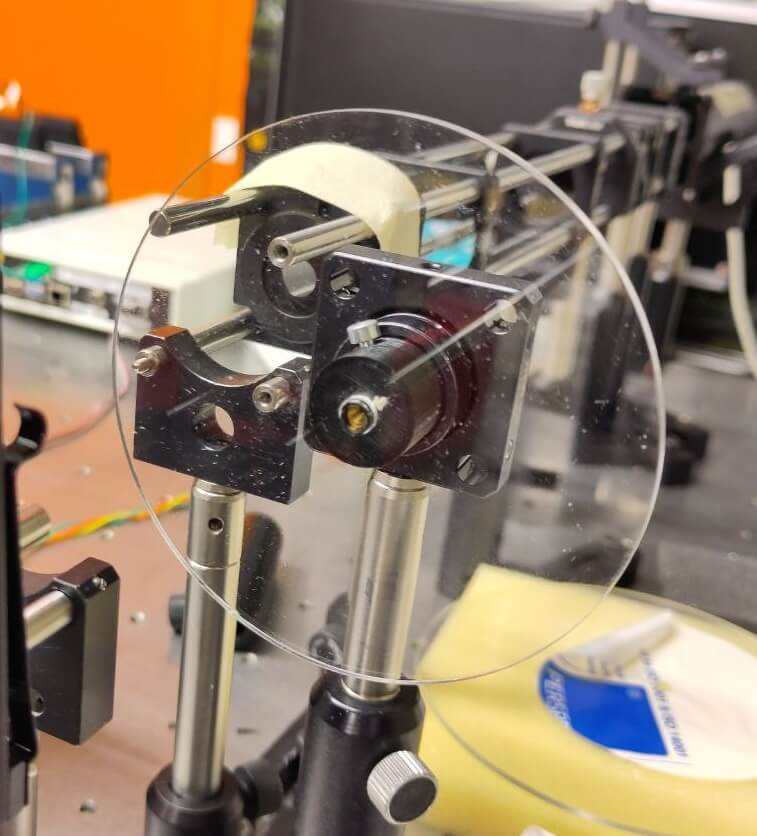
\includegraphics[width=0.5\textwidth]{assets/figures/ameliorations/disque_fixe.jpeg}
              \caption{Disque placé dans le faisceau}\label{fig:disque_fixe}
          \end{figure}

    \item Attendre quelques secondes que la mesure sur le logiciel soit stable:
          %   \begin{figure}[H]
          %       \centering
          %       
\includegraphics[width=0.5\textwidth]{assets/figures/Placeholder.jpeg}
          %       \caption{Placeholder}\label{Placeholder}
          %   \end{figure}

    \item Prendre la mesure l'enregistrer en format \textbf{.csv} avec le numéro de mesure.

    \item Tourner le disque d'un petit angle:
          \begin{figure}[H]
              \centering
              \includegraphics[width=0.5\textwidth,trim = 0 140 0 0, clip]{assets/figures/ameliorations/écran_rotation_manuelle.png}
              \caption{Rotation manuelle de l'écran}\label{fig:rotation_manuelle}
          \end{figure}
\end{enumerate}

Répéter en suite les étapes \textbf{2 à 4} pour autant de mesures qu'il le faut.
Dans le cadre de ce projet, plus il y a de données mieux c'est, il convient donc d'automatiser le
processus de prise de mesure au maximum pour pouvoir caractériser les écrans de turbulance facilement.

\subsection{Solution développée}
L'idée est de contrôler par ordinateur la prise de mesure ,interaction avec la caméra et la rotation de l'écran.
Après une petite configuration, l'utilisateur doit pouvoir laisser le système tourner et prendre les mesures nécessaires sans
interaction externe nécessaire.

\subsubsection{Caméra}

La caméra utilisée pour mesurer le front d'ondes est une \textbf{Thorlabs WFS40-7AR}:
\begin{figure}[H]
    \centering
    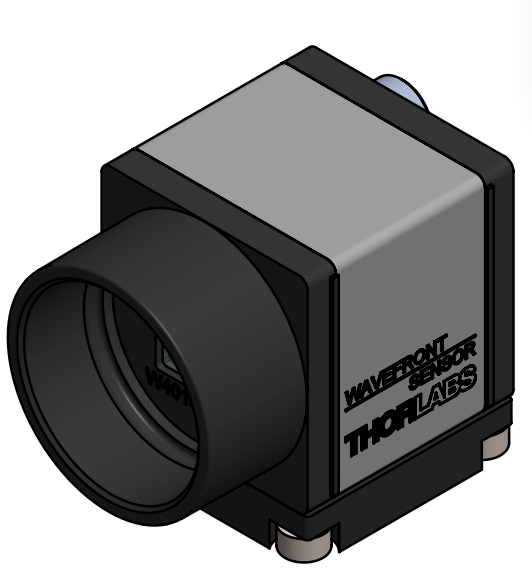
\includegraphics[width=0.4\textwidth]{assets/figures/ameliorations/thorlabs_40_7AR.png}
    \caption[Image de la caméra Thorlabs]{Image de la caméra Thorlabs \autocite{Camera_thorlabs_photo}}\label{fig:camera_thorlabs}
\end{figure}

Comme dit précédemment, il est possible d'intéragir avec la caméra à l'aide du logiciel fourni par Thorlabs, ce dernier permet de régler
la caméra, lire différentes mesures et visualiser le front d'onde.

La problématique était donc de trouver un moyen de communiquer avec la caméra, hors du logiciel dédié pour créer le programme de mesures.
Le manuel de la caméra, parle de la possibilité d'utiliser \textbf{LabView} pour accéder aux données et contrôler la caméra, en effet des
drivers spécifiques sont installés avec le programme de Thorlabs. Malheureusement cette solution ne fut pas retenue pour les raisons suivantes:

\begin{itemize}
    \item Le système de liscence de LabView à l'école est très contraignant.
    \item Mon système d'exploitation principal est MacOs (ainsi que celui de M. Jolissaint), LabView est peu compatible avec Mac et l'emulation de windows crash à cause des drivers.
\end{itemize}

Cela a donc porté mon regard sur l'utilisation de \textbf{Matlab}, et par chance, un utilisateur a développé une librairie Matlab permettant d'utiliser la caméra ! Cette ressource est disponible ici :
\url{https://www.mathworks.com/matlabcentral/fileexchange/116485-driver-for-thorlabs-shack-hartmann-wavefront-sensors-wfs}, elle a comme pré-requis, l'installation du logiciel de Thorlabs pour accéder aux drivers.

Il faut donc toujours utiliser un ordinateur sous windows, mais Matlab étant plus simple au niveau de ses licenses, il a été plus simple de juste travailler sur l'ordinateur du laboratoire.

\subsubsection{Rotation et translation de l'écran}
Pour faire tourner l'écran il fallait :
\begin{itemize}
    \item Un moyen de faire tourner l'écran.
    \item Faire communiquer l'ordinateur et le moyen de rotation.
\end{itemize}

Pour répondre au 1er besoin, nous avons utilisé un moteur pas-à-pas \textbf{28byj-48} :
\begin{figure}[H]
    \centering
    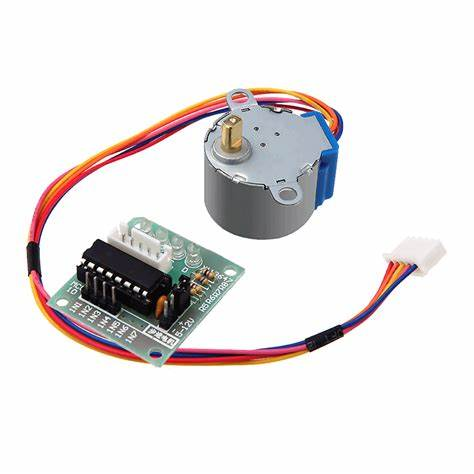
\includegraphics[width=0.5\textwidth]{assets/figures/ameliorations/stepper.jpeg}
    \caption[Moteur 28byj-48 pas-à-pas et son driver]{Moteur 28byj-48 pas-à-pas et son driver \autocite{photo_28byj-48}}
\end{figure}

Concernant la translation de l'écran, nous avons choisi d'utiliser un moteur pas-à-pas classique \textbf{36H22HM-0404A15-Z} avec un pignon et une crémaillère basée sur les
dimensions d'une courroie MXL classique\cite{dimensions_courroies_mxl}\footnotemark :
\begin{figure}[H]
    \centering
    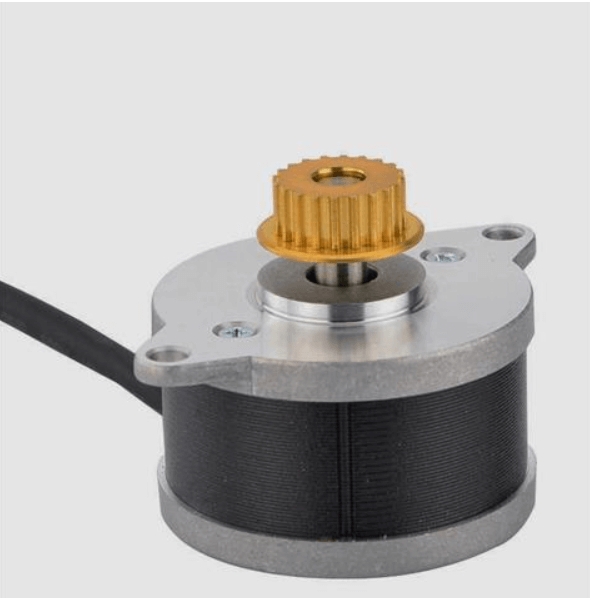
\includegraphics[width=0.3\textwidth]{assets/figures/ameliorations/36H22HM-0404A15-Z.png}
    \caption[Moteur 36H22HM-0404A15-Z]{Moteur pas-à-pas 36H22HM-0404A15-Z\autocite{moteur_translation_site}\footnotemark}
\end{figure}

\begin{figure}[H]
    \centering
    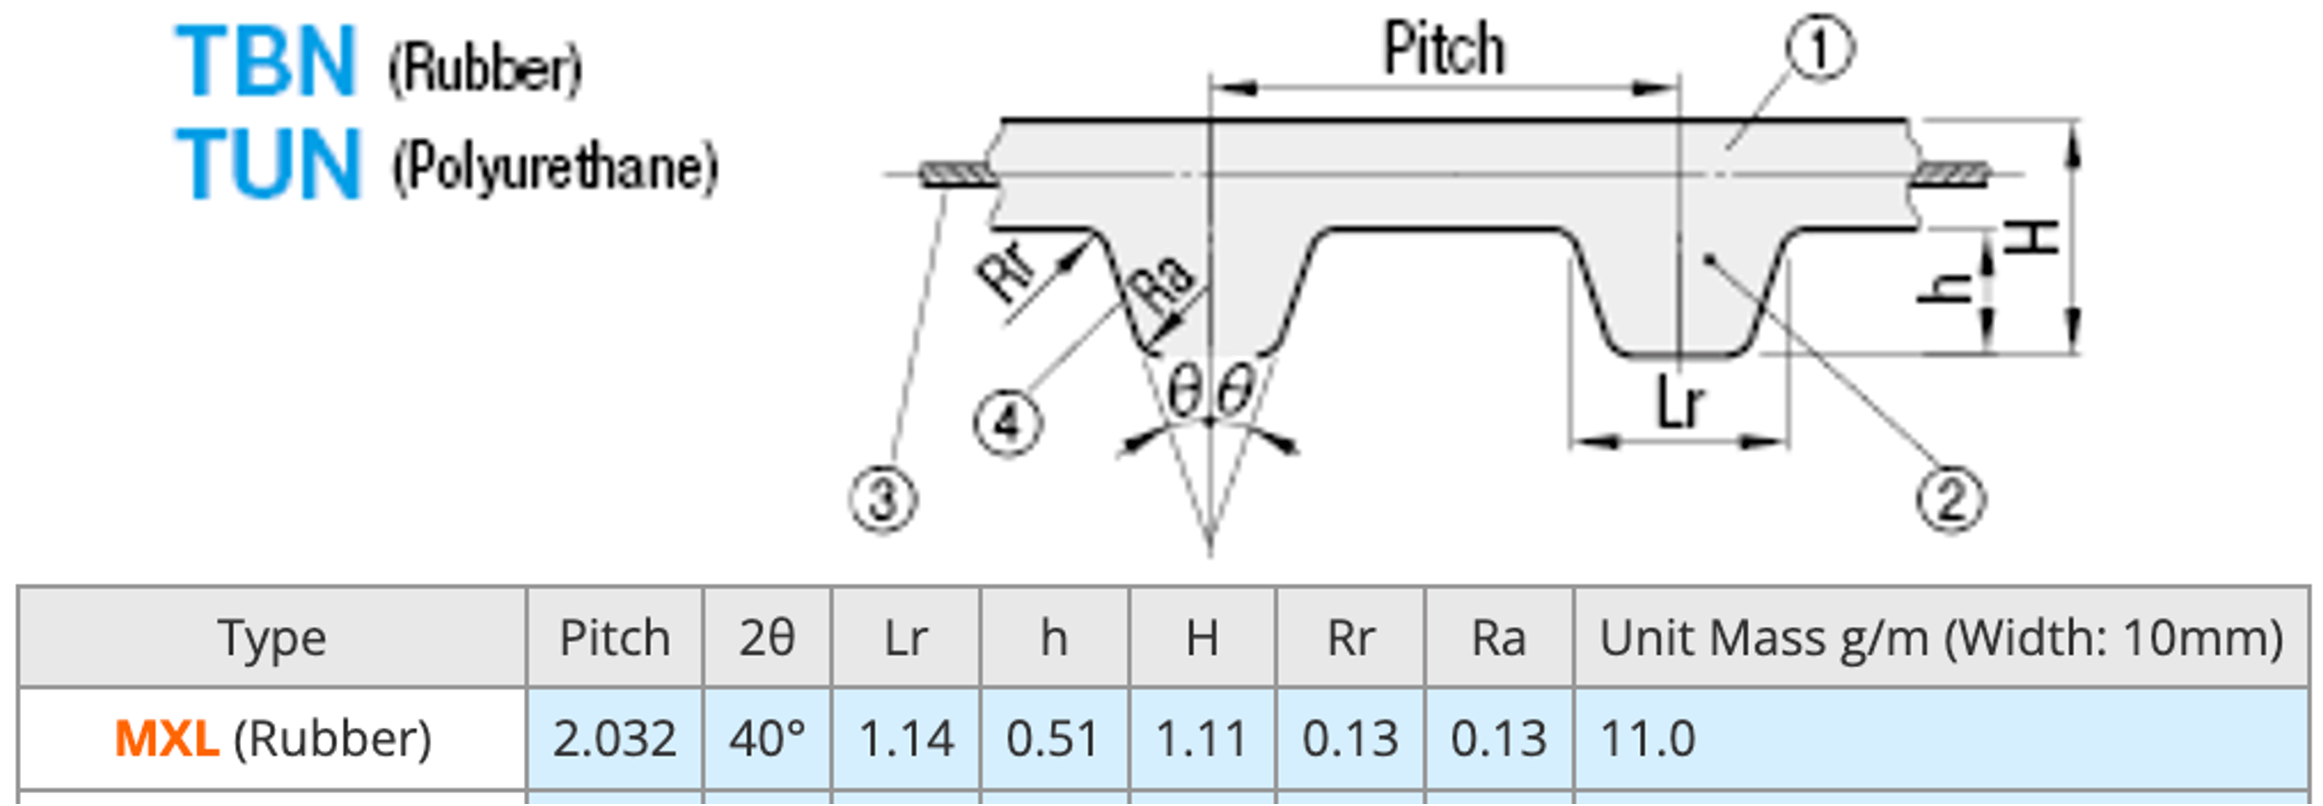
\includegraphics[width=0.8\textwidth]{assets/figures/ameliorations/dimensions_cremaillere.png}
    \caption[Dimensions crémaillère]{Dimensions crémaillère\autocite{dimensions_courroies_mxl}}
\end{figure}

\footnotetext{\url{https://uk.misumi-ec.com/vona2/detail/110302566050/}}
\footnotetext{\fullcite{moteur_translation_site}}



\subsubsection{Communication entre ordinateur et arduino}

Pour la communication entre l'ordinateur, le moteur de translation et celui de rotation, un arduino nano (clône) est utilisé :
\begin{figure}[H]
    \centering
    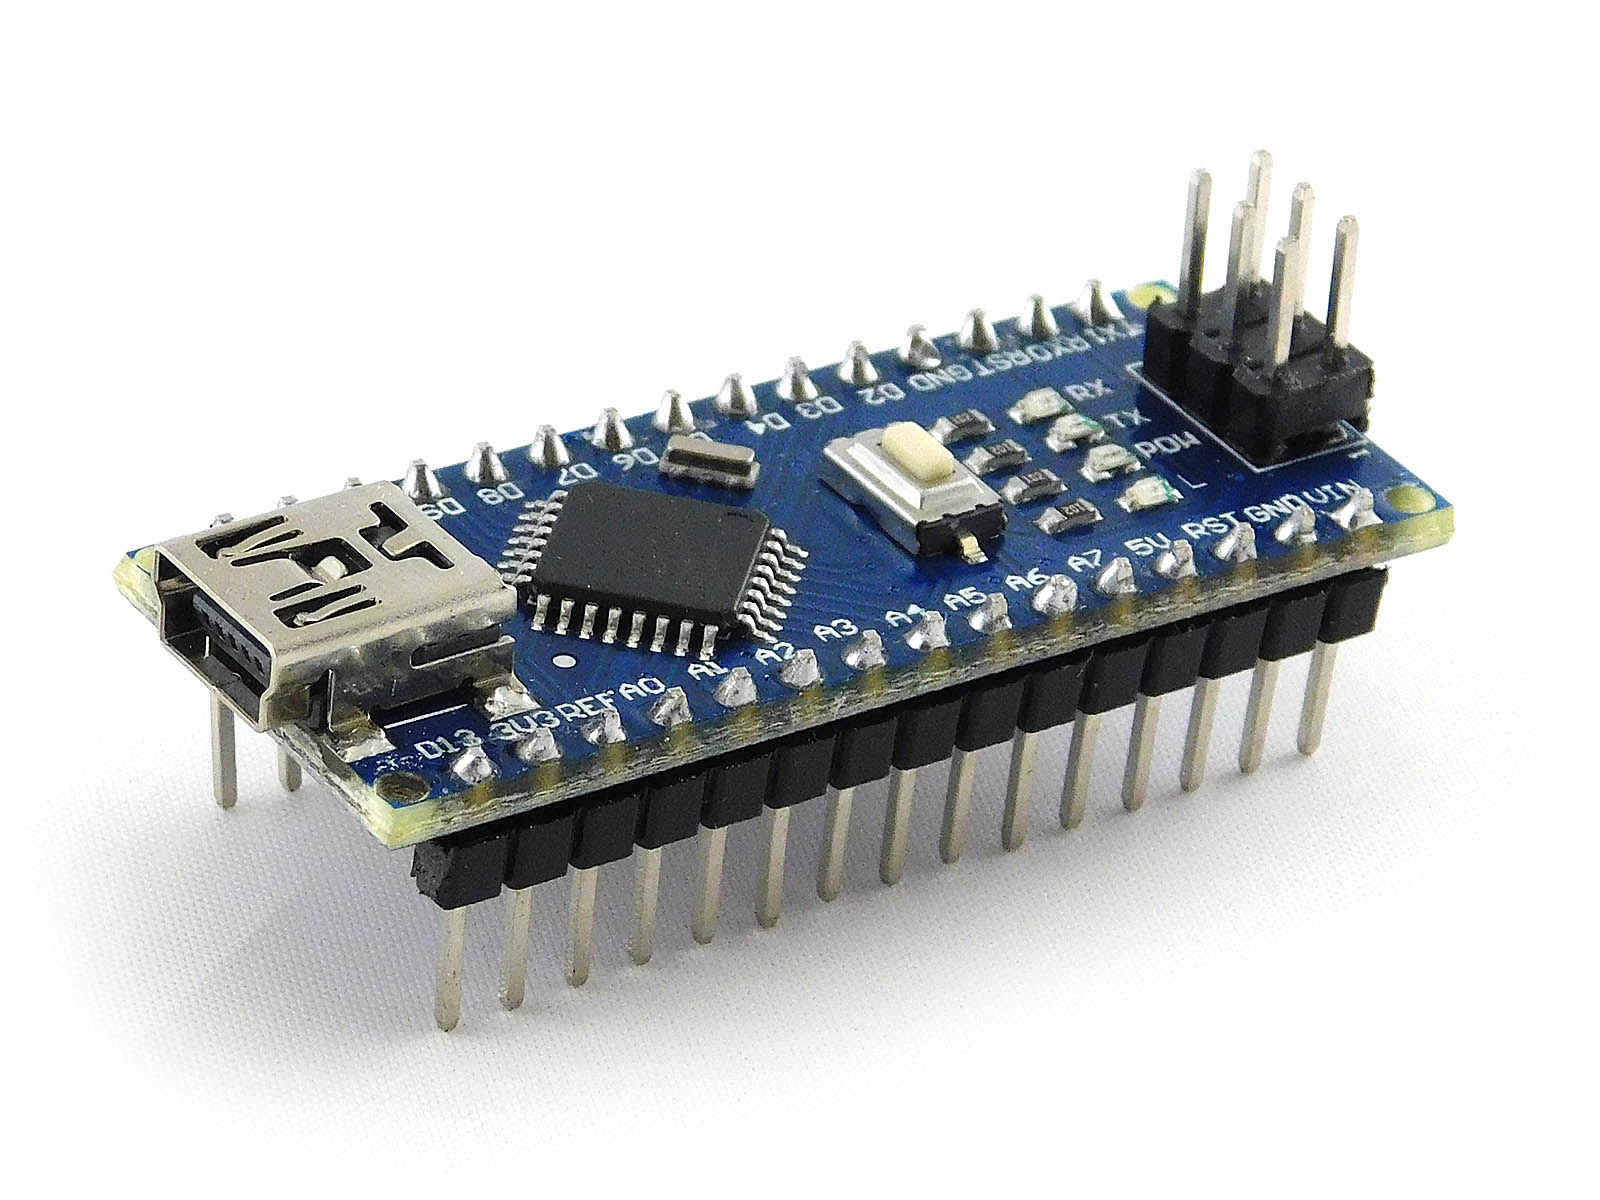
\includegraphics[width = 0.4\textwidth]{assets/figures/ameliorations/arduino_nano.jpg}
    \caption[Exemple de clône d'arduino nano]{Exemple de clône d'arduino nano \autocite{clone_nano}}
\end{figure}

Pour faire fonctionner le driver \textbf{ULN2003} du moteur de rotation à l'aide du microcontrôleur, la librairie \textbf{AccelStepper}\autocite{librairie_accelstepper} est utilisée.
Cette dernière permet entre autre, de régler l'accélération du moteur et le nombre de pas à effectuer, de démarrer le mouvement et de l'arrêter, savoir combiens de pas il reste à faire et bien plus,
la documentation du la librairie n'étant pas claire aux premiers abords un ressource complémentaire fut utilisée \autocite{AccelStepper_manual}.

Pour le moteur de translation, un driver \textbf{DRV8825} est employé :

\begin{figure}[H]
    \centering
    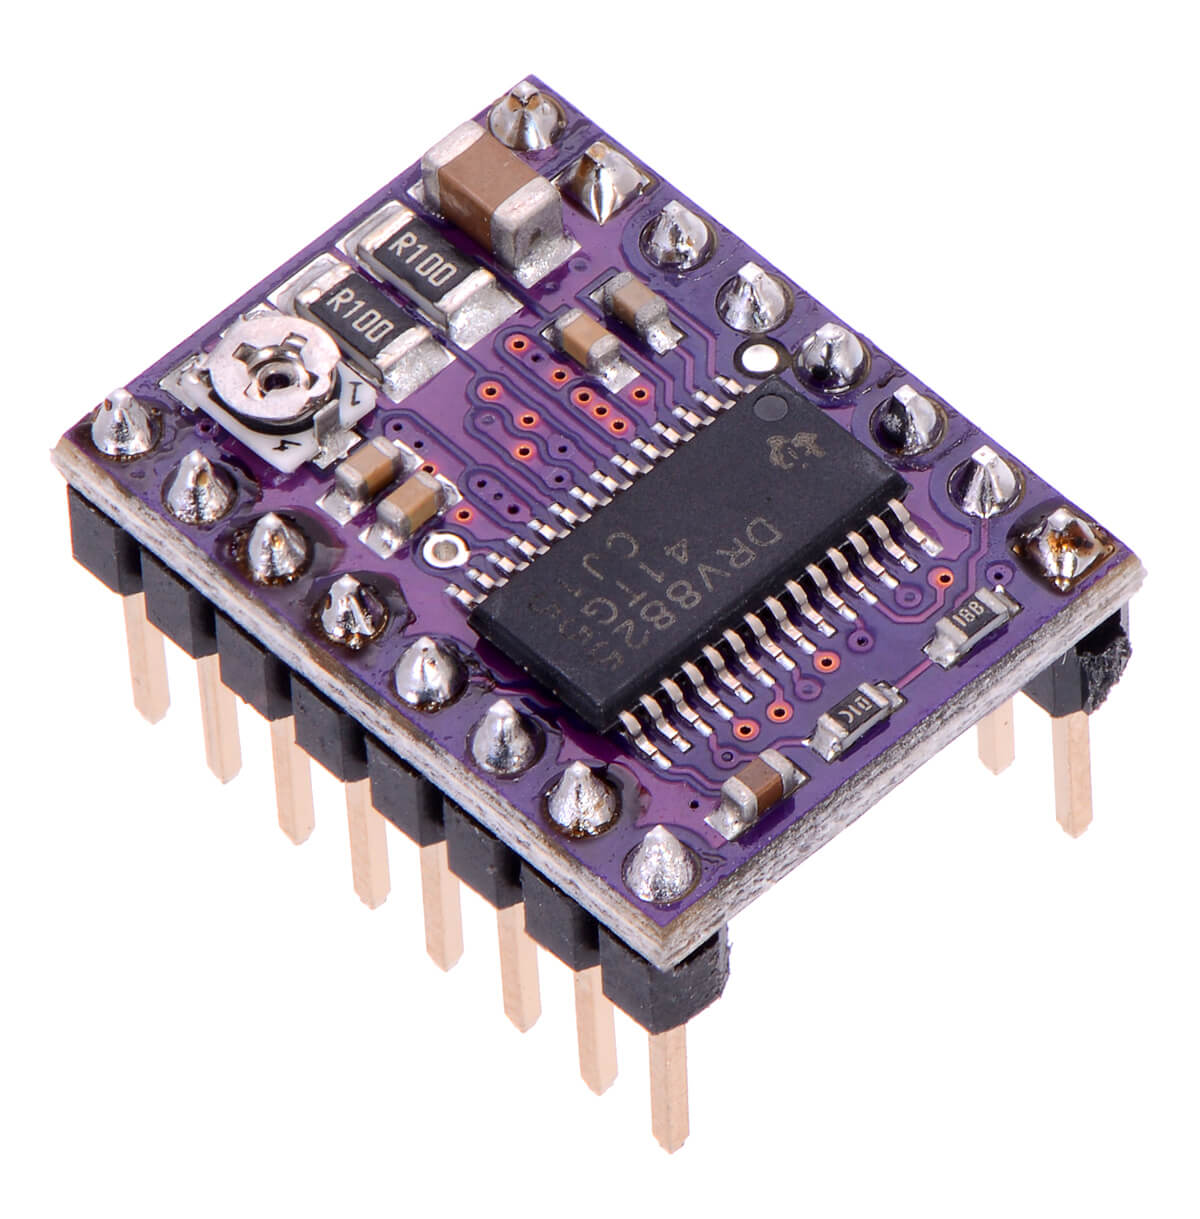
\includegraphics[width = 0.2\textwidth]{assets/figures/ameliorations/drv-8825.jpg}
    \caption[Driver DRV8825]{Driver DRV8825 \autocite{driver_DRV8825}\footnotemark}
\end{figure}
\footnotetext{\fullcite{driver_DRV8825}}
Ce dernier est piloté à l'aide de la librairie \textbf{StepperDriver}\cite{stepperDriver_lib}\footnotemark.

\footnotetext{\fullcite{stepperDriver_lib}}

La communication de matlab au microcontrôleur se fait via interface serial usb !
Le principe du protocole de communication est le suivant :
\begin{figure}[H]
    \centering
    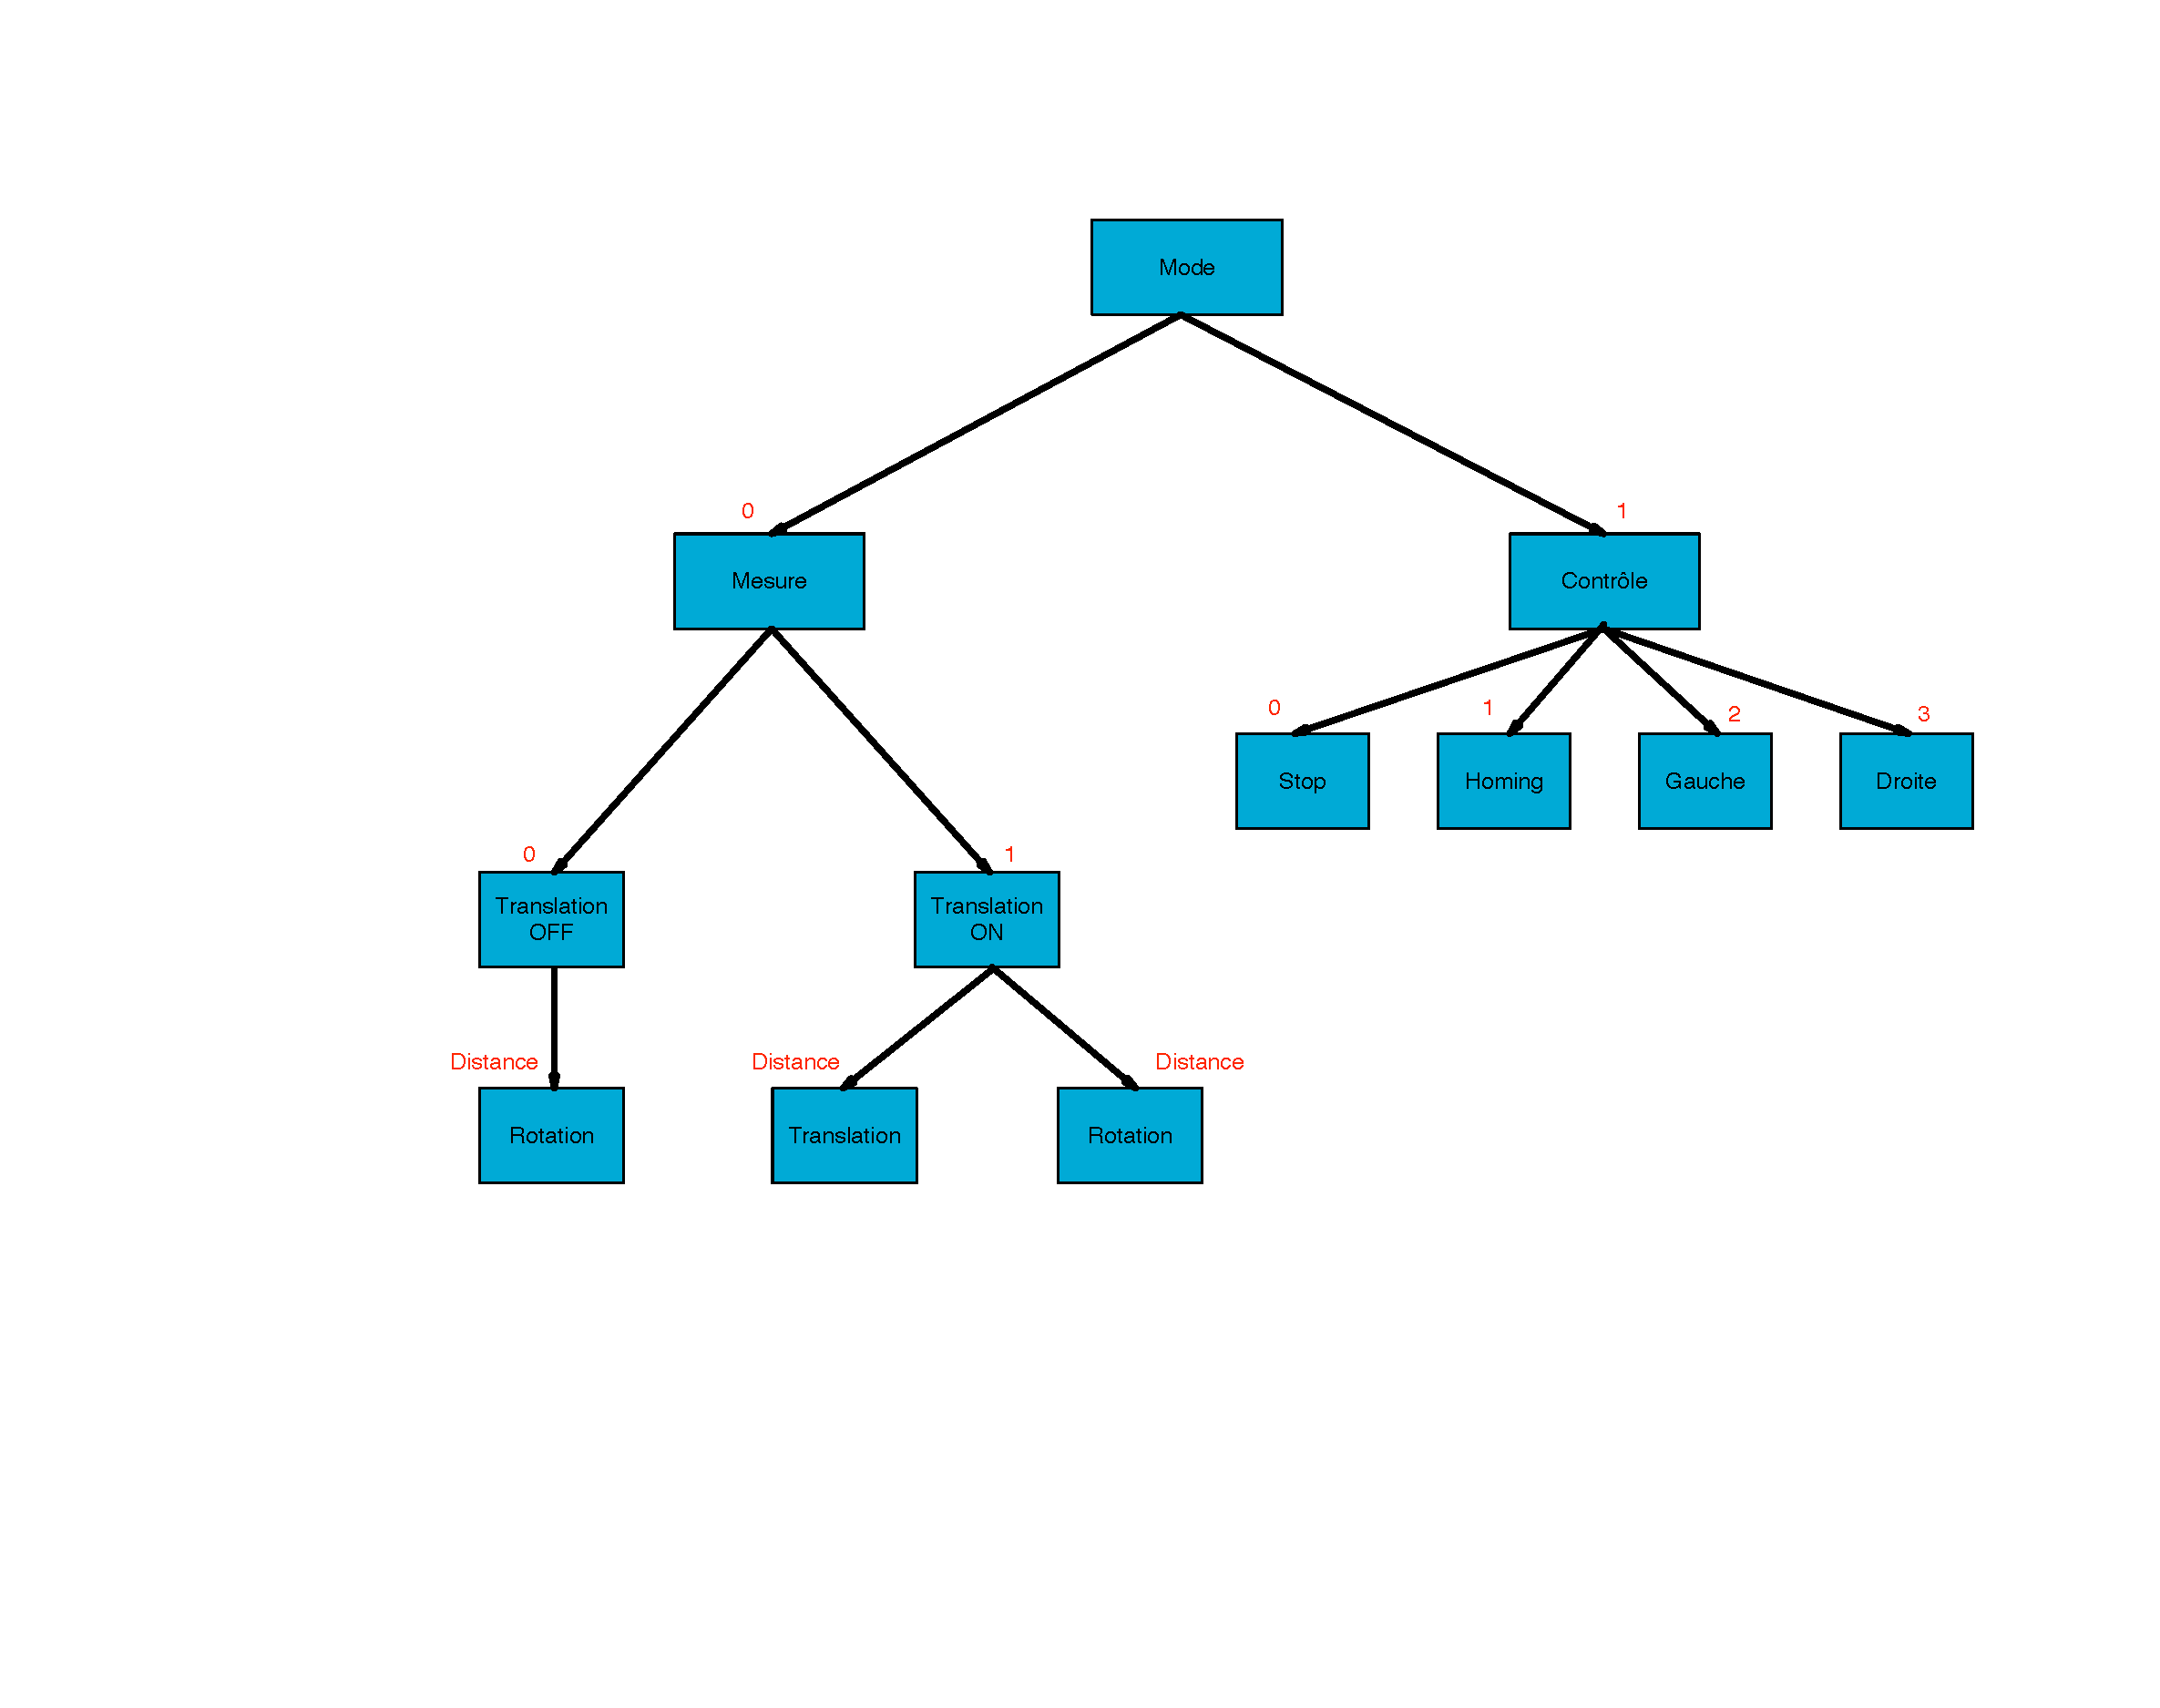
\includegraphics[page = 1, width = \textwidth, trim = {7cm 9cm 2cm 3cm},clip]{assets/figures/ameliorations/trame_comm.pdf}
    \caption[Structure de communication]{Structure de communication sous forme de choix ( en \color{red} rouge \color{black} = valeur dans la trame)}
\end{figure}
Sous forme de trame cela donne donc :
\begin{figure}[H]
    \centering
    
\includegraphics[width = 0.8\textwidth]{assets/figures/ameliorations/trame comm.png}
    \caption[Trame ordinateur <-> arduino mesure]{Trame ordinateur <-> arduino mesure( en \color{red} rouge \color{black} = valeur dans la trame)}
\end{figure}

Donc par exemple pour déclencher un homing la trame envoyée sera :
\begin{figure}[H]
    \centering
    
\includegraphics[scale = 1.3]{assets/figures/ameliorations/trame_homing.png}
    \caption[Trame homing]{Trame de homing}
\end{figure}
Ou pour effectuer une rotation de 130 pas et une translation de 150 pas (si on a fait un tour complet d'écran), la trame est la suivante:
\begin{figure}[H]
    \centering
    
\includegraphics[scale = 1.2]{assets/figures/ameliorations/trame_translation_rotation.png}
    \caption[Trame translation rotation]{Trame de translation et de rotation pour mesure de l'écran\label{fig:trame_trans_rota}}
\end{figure}

Les trames sont quant à elles envoyées dans le bus serial sous forme de string de valeurs séparées par des virgules, par exemple pour la trame
de la \autoref{fig:trame_trans_rota} cela donnerait: \textbf{0,1,150,130}.

L'arduino qui reçoit ces instructions fonctionne sous le principe suivant :

\begin{figure}[H]
    \centering
    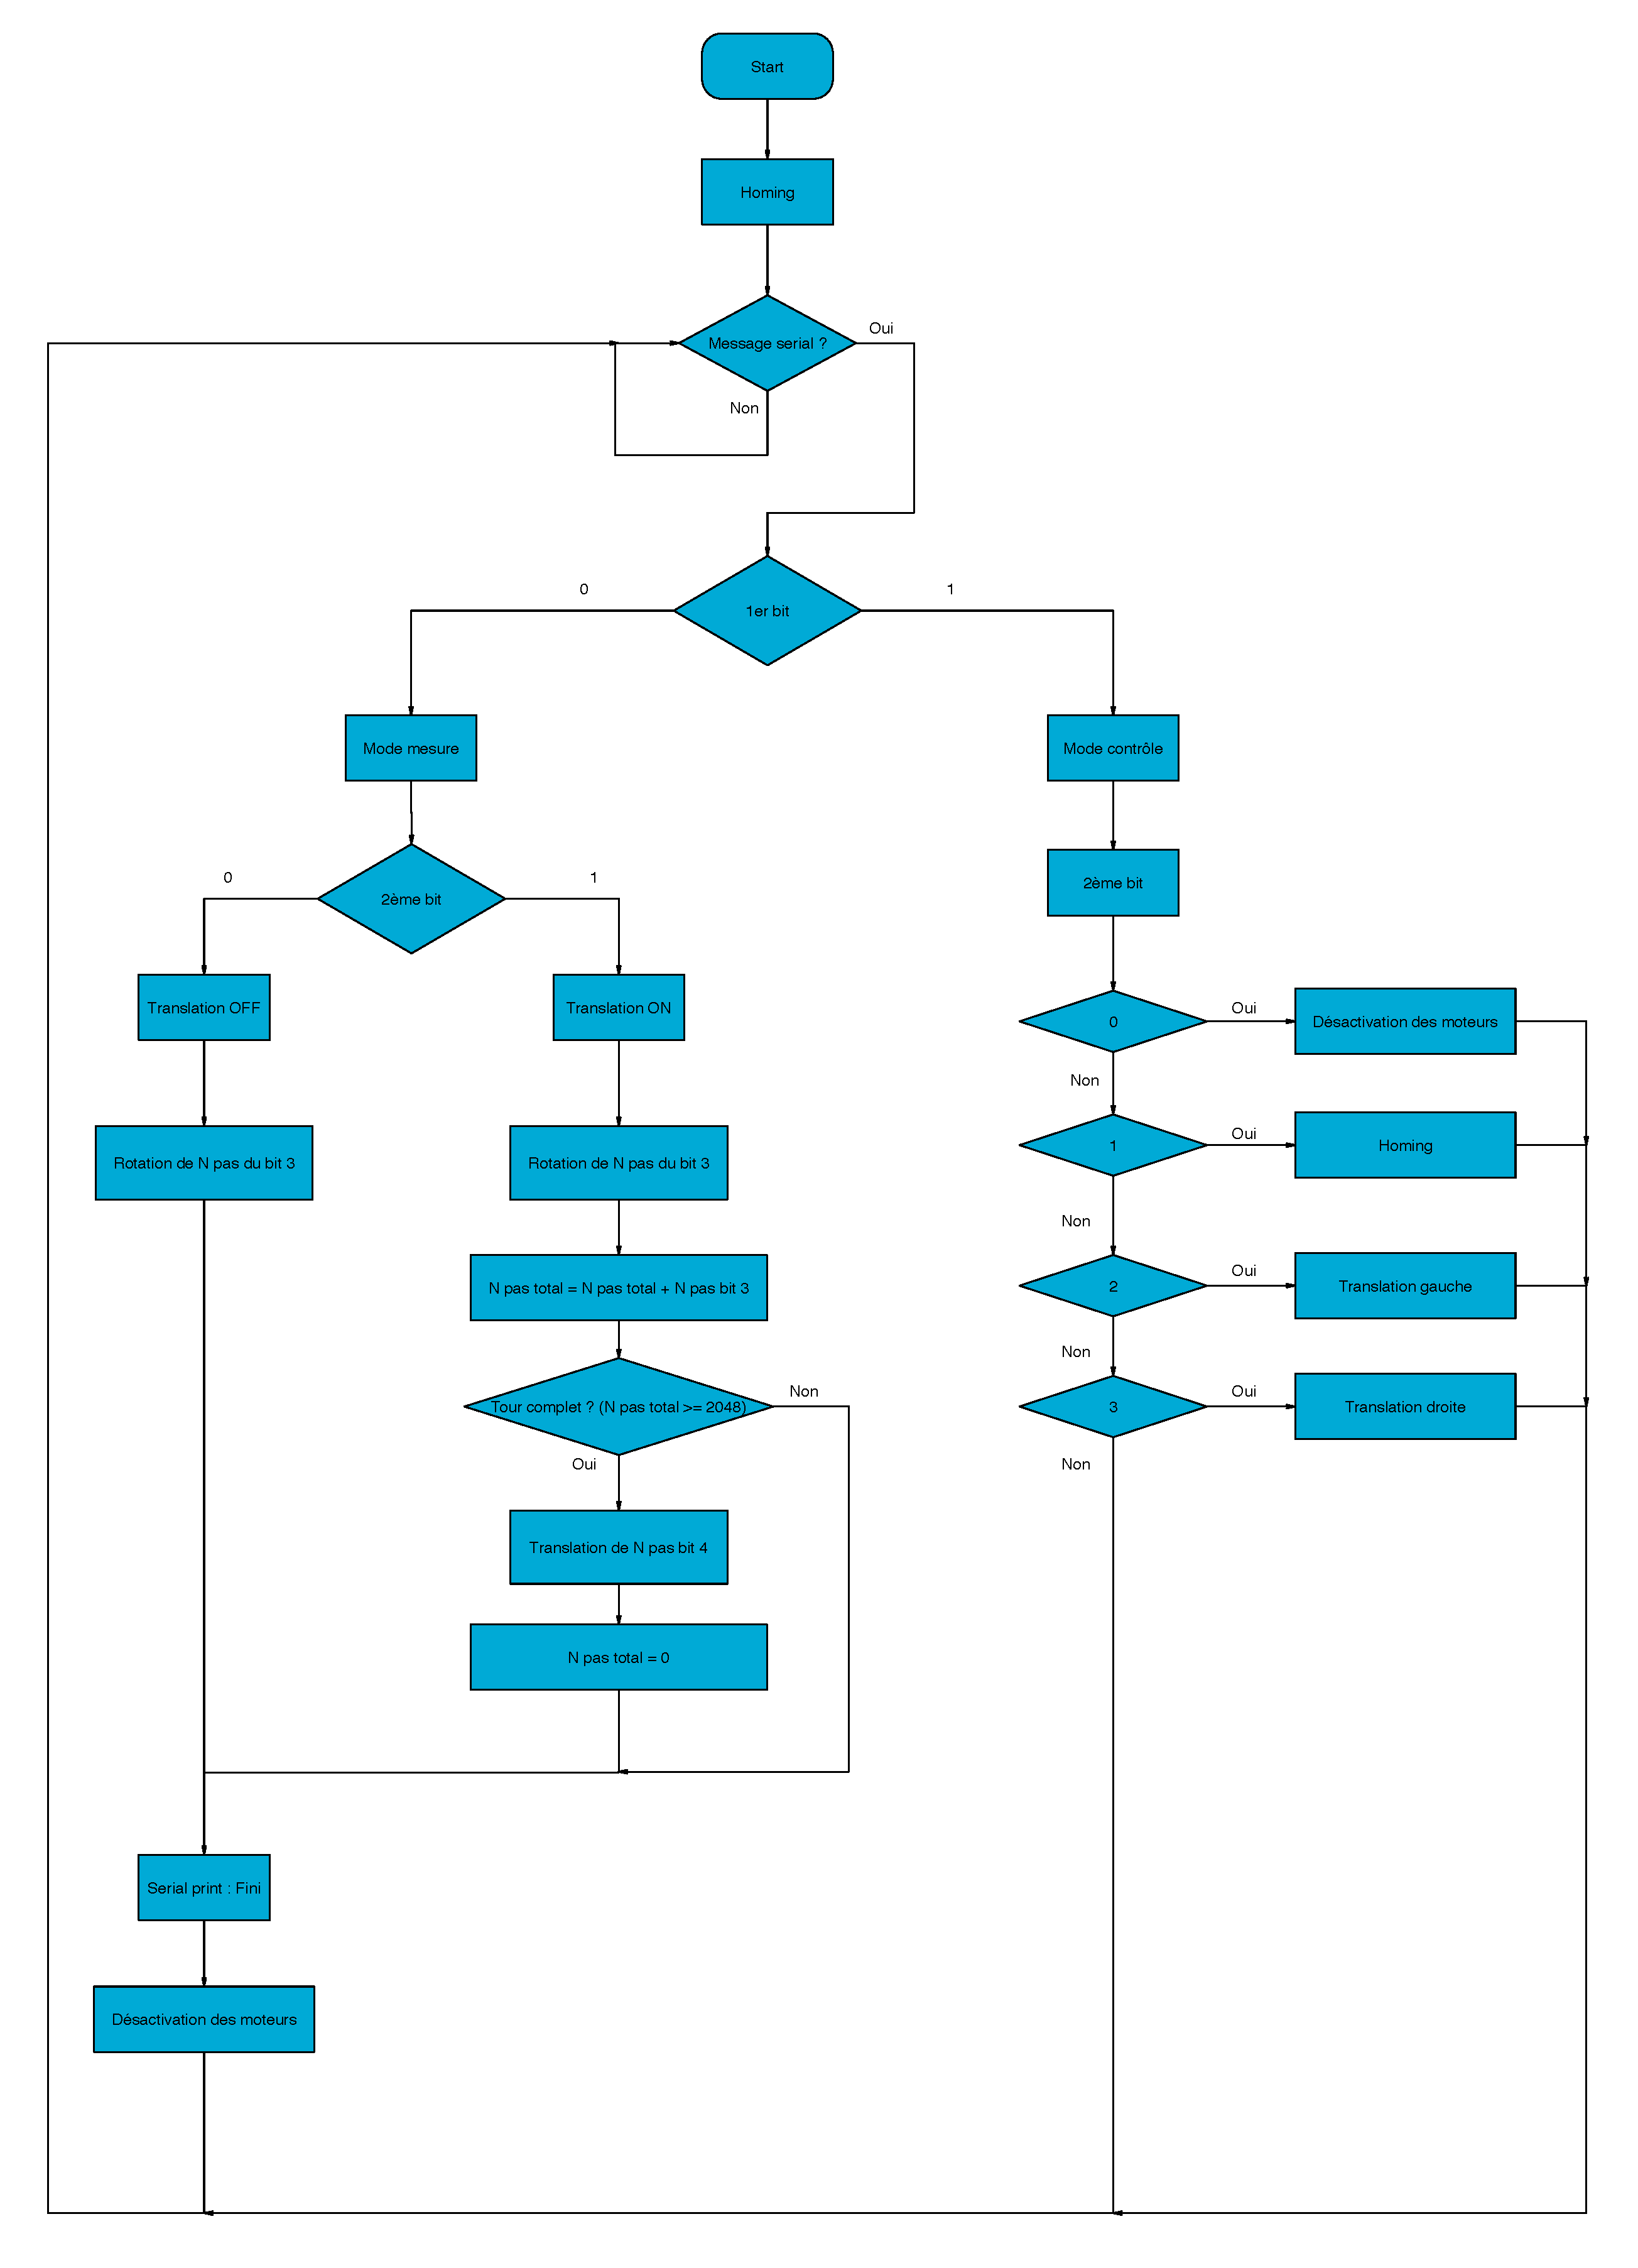
\includegraphics[width = \textwidth]{assets/figures/ameliorations/Structogramme_arduino.pdf}
    \caption[Structogramme programme microcontrôleur de mesure]{Structogramme programme microcontrôleur de mesure}
\end{figure}
Le code de l'arduino est consultable en \autoref{code:arduino_mesure}.

\newpage
\subsection{PCB système de mesure}

\begin{figure}[H]
    \centering
    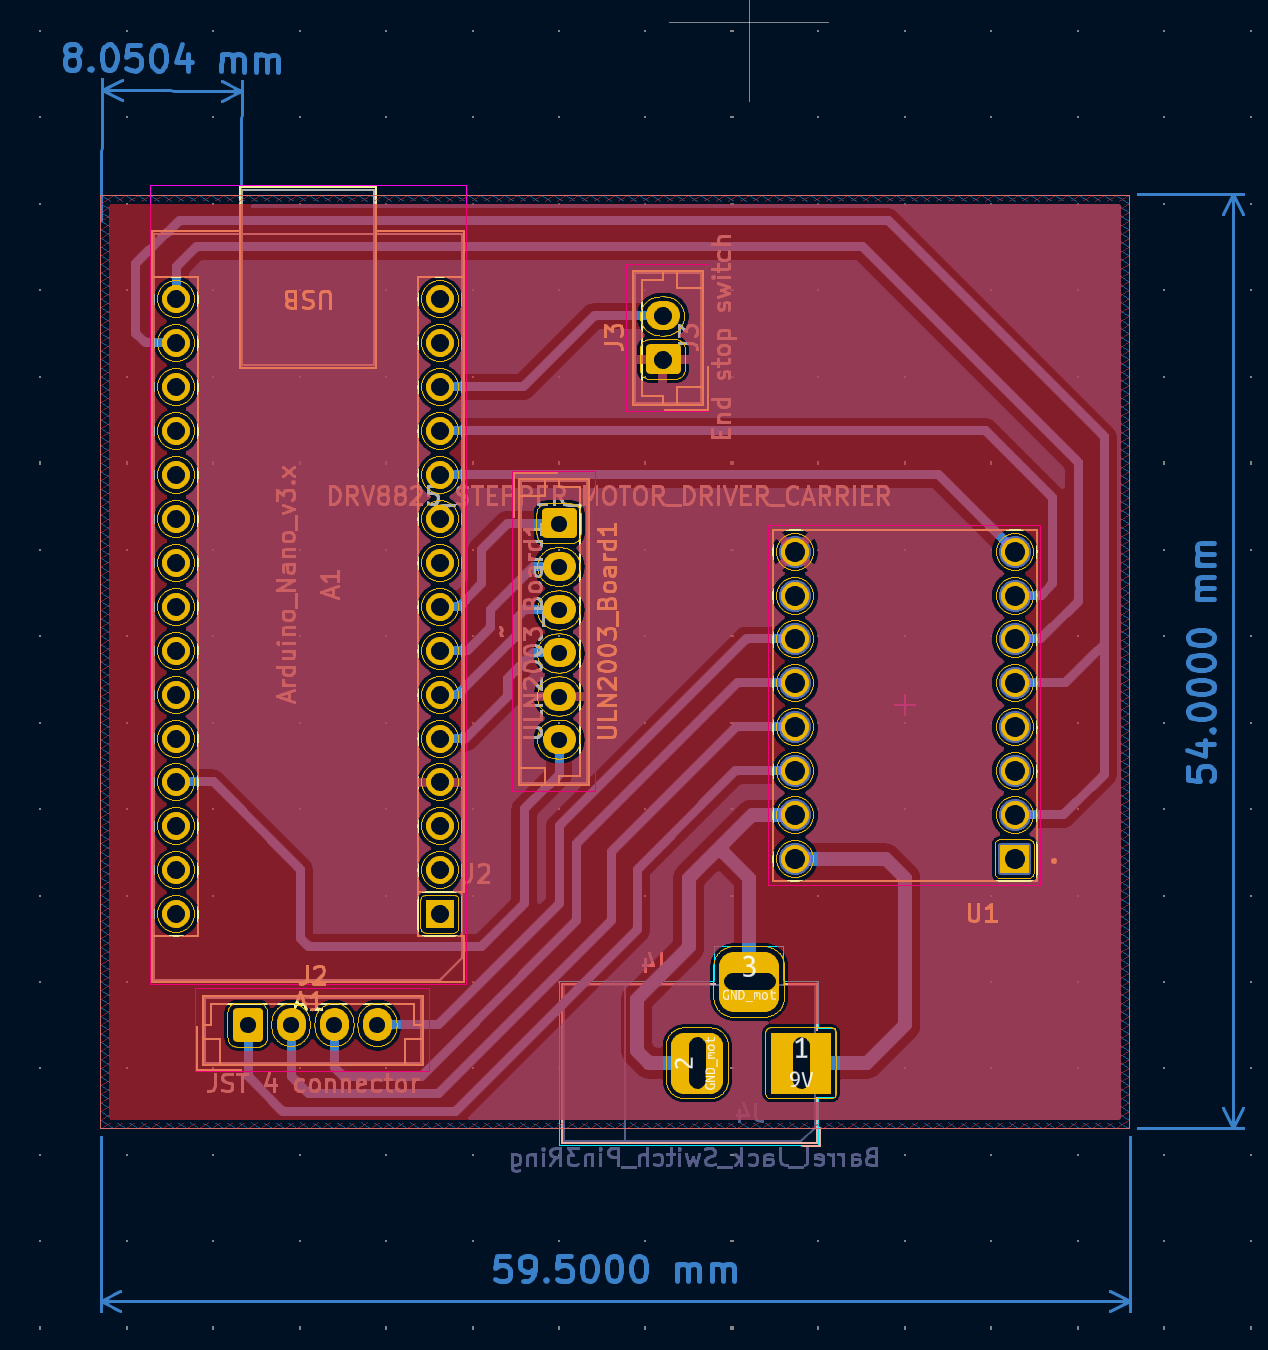
\includegraphics[width = \textwidth]{assets/figures/ameliorations/PCB_rotation_translation.png}
    \caption[PCB du système de mesure]{PCB du système de mesure (diagramme électrique disponible en \autoref{PCB:mesure})}
\end{figure}

\newpage
Le PCB réalisé au sein de l'école est populé de la façon suivante:

\begin{figure}[H]
    \centering
    \includegraphics[width = \textwidth]{assets/figures/ameliorations/PCB_mesure_Annoté.png}
    \caption[Photo du PCB du système de mesure]{Photo du PCB du système de mesure}
\end{figure}

La liste des pièces pour populer ce PCB est la suivante :
\begin{itemize}
    \item 1 - Arduino Nano - ici un Vellman WPB102
    \item 1 - switch de fin de course
    \item 1 - driver drv8825
    \item 1 - alimentation 9V
    \item 1 - Moteur 28byj-48 et sa board ULN2003
    \item 1 - Moteur 36H22HM-0404A15-Z
    \item 1 - connecteur femmelle JST 6 pin pas de 2.54mm
    \item 1 - Connecteur femelle JST 4 pin pas de 2.54mm
    \item 1 - Connecteur mâle cavalier 2 pin
\end{itemize}

À noter que le connecteur du moteur de translation possède un adaptateur, ceci est dû à une erreur de conception, cette erreur est corrigée
dans les fichiers fournis en annexe.

Concernant le driver drv 8825, il convient de régler la limite de courant que sera envoyée au moteur pas-à-pas, la marche à suivre est trouvable \href{https://www.pololu.com/product/2133}{ici}.\footnotemark

\footnotetext{\href{https://www.pololu.com/product/2133}{https://www.pololu.com/product/2133}}


\subsection{Machine de mesure}
Pour acceuillir le PCB et ses organes, il a donc fallu développer le système suivant :
\begin{figure}[H]
    \centering
    \includegraphics[width = \textwidth,trim={1cm 5cm 2cm 6cm},clip]{assets/figures/ameliorations/système_mesure_front.jpeg}
    \caption{Photo du système de mesure final}
\end{figure}

\newpage

\subsubsection{Fonctionnement}
Passons en revue le fonctionnement de la fonction de translation:
\begin{figure}[H]
    \centering
    \includegraphics[width = \textwidth]{assets/figures/ameliorations/3D_fonctionnement_crémaillère.png}
    \caption{Image du système de translation}
\end{figure}
La crémaillère est la partie fixe du système qui est reliée à la table optique, le pignon en tournant va alors décaler l'entièreté du système de mesure
vers la gauche ou la droite.

Le switch de fin de course sert à la fonction de homing du système, cela correspond à la position la plus à l'intérieur du disque
de phase pour le laser, en suite le système peut se déplacer sur une course de 4cm.

Concernant les resorts de compression, ils sont la pour assurer que la crémaillère ne "déraille" pas et que les dents du pignon rèstent bien plaquées
contre cette dernière, la plaque de pression est réglable en hauteur à l'aide de deux vis.

\newpage
\subsubsection{Réglage crémaillère}
\begin{figure}[H]
    \centering
    \includegraphics[width = \textwidth]{assets/figures/ameliorations/réglage_crémaillère_système_mesure.jpg}
    \caption{Réglage de la crémaillère lors du montage}
\end{figure}
Avant de fixer totalement le moteur du pignon, il faut bien veiller à ce que le système de crémaillère est bien réglé.
Comme on peut le voir sur la figure de gauche, il faut que le guide du support à crémaillère soit bien plaqué dans la rainure
de guidage du système de mesure, en suite comme sur l'image de droite, on peut alors régler la position verticale du pignon
pour que les dents de ce dernier et celle de la crémaillère soit bien en contact. Après cela, il conviendra d'ajuster la plaque de
pression pour bien maintenir le tout.

\subsubsection{Fixation de l'écran}
L'écran se fixe sur la machine de mesure à l'aide d'une vis à main :
\begin{figure}[H]
    \centering
    \includegraphics[width = \textwidth]{assets/figures/ameliorations/fixation_écran.png}
    \caption{Système de fixation de l'écran}
\end{figure}
À noter que les trous taraudés sont à faire à la main à l'aide d'un tourne à gauche directement dans le plastique, en effet,
cela est suffisement solide car l'utilisateur n'est pas censé démonter le moteur de rotation à chaque utilisation de la machine.

\subsubsection{Fixation du système de mesure au banc optique}
Le support à crémaillère vient se fixer sur un support de table optique à l'aide d'une vis sans tête m6 :
\begin{figure}[H]
    \centering
    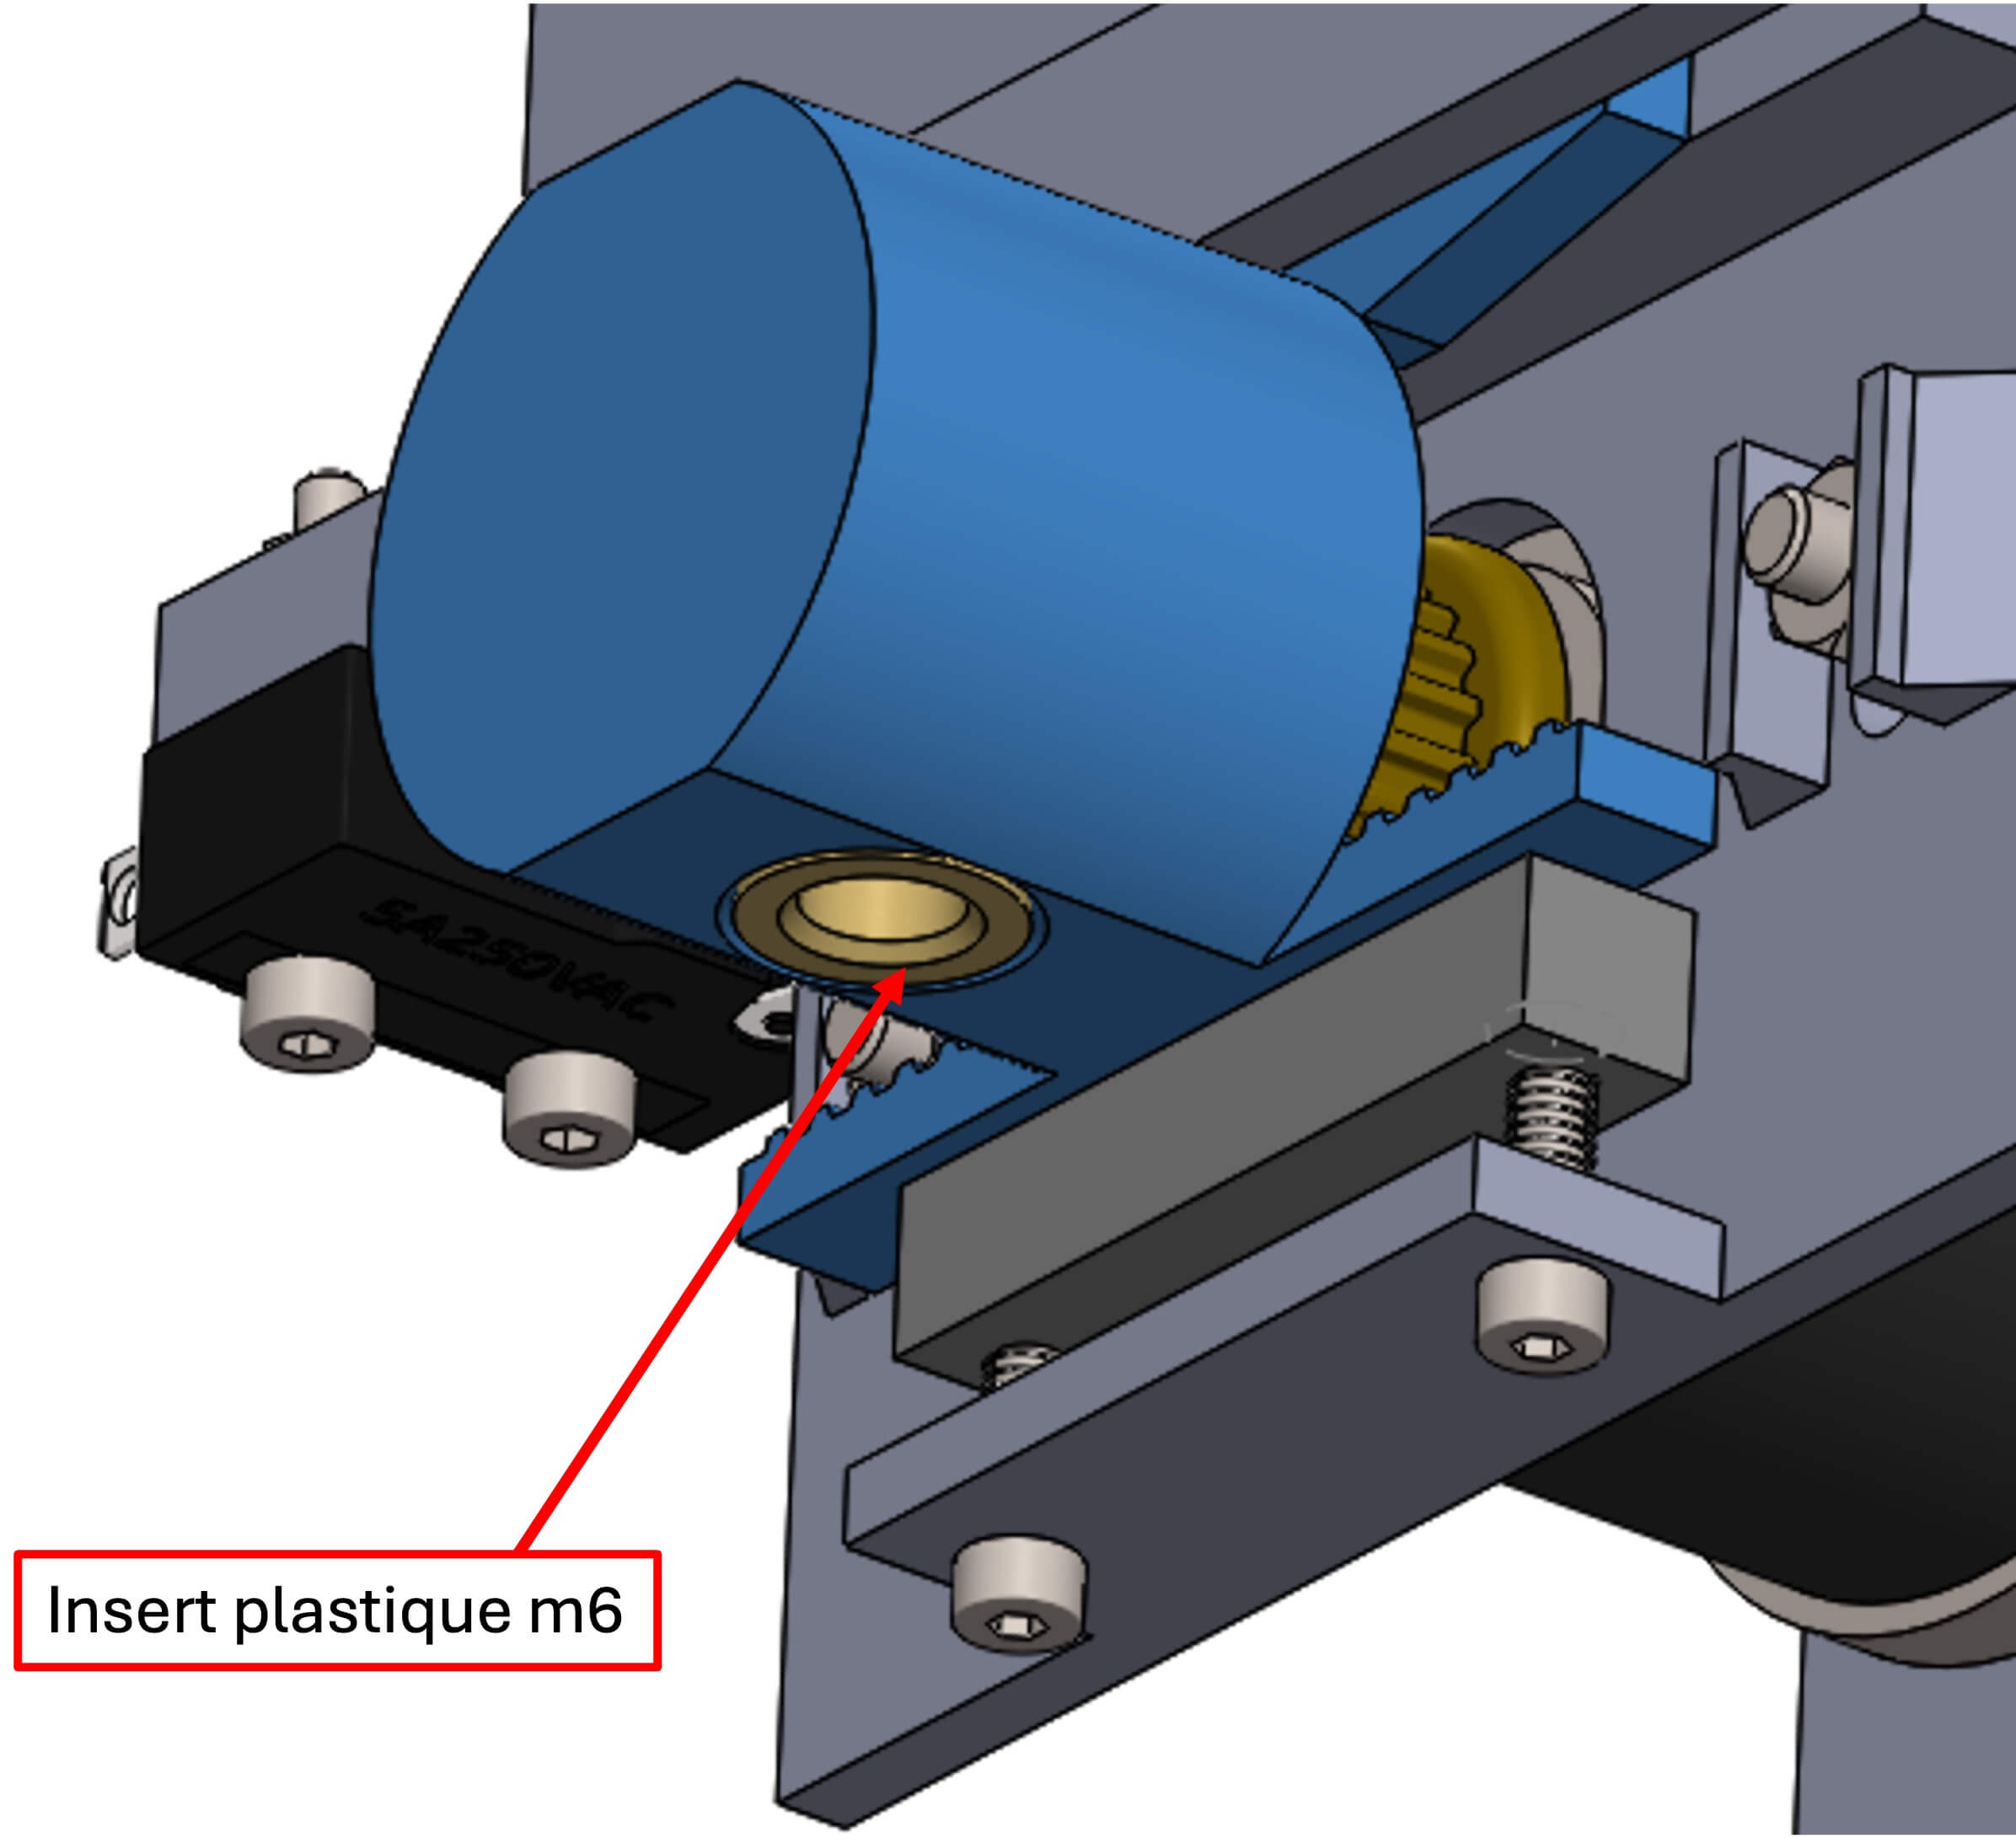
\includegraphics[width = 0.5\textwidth]{assets/figures/ameliorations/fixation_table_optique.jpg}
    \caption{Fixation du système de mesure à la table optique}
\end{figure}
\begin{figure}[H]
    \centering
    \includegraphics[width = 0.6\textwidth,trim = {0 2cm 3cm 3cm},clip]{assets/figures/ameliorations/système_mesure_back.jpeg}
    \caption{Photo du système sur un support de table optique}
\end{figure}

\newpage
\subsubsection{Fabrication du système de mesure}
Le système de mesure a été conçu avec l'impression 3D en tête, dans cette sous section, nous allons décrire quelques recommandation pour imprimer les pièces.
Pour la pièce principale, il est recommandé de l'imprimer dans cette orientation :

\begin{figure}[H]
    \centering
    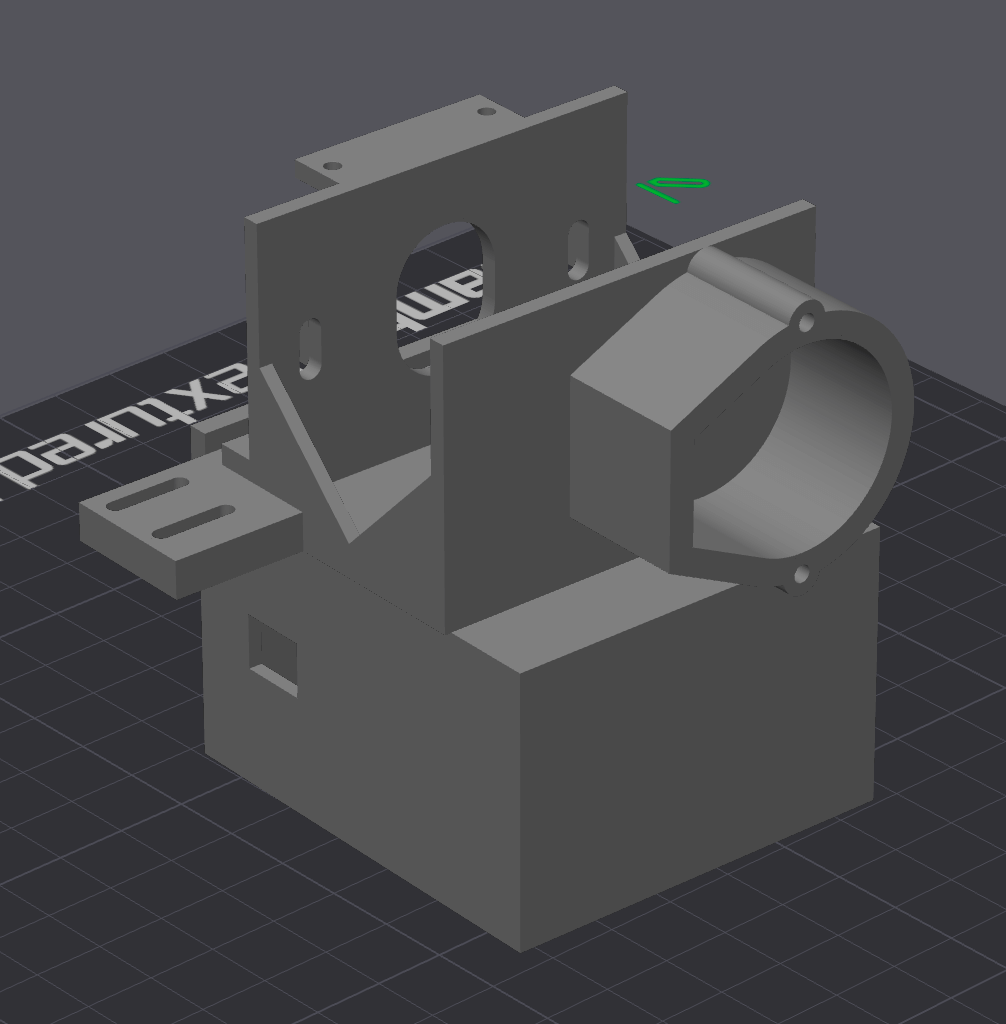
\includegraphics[width = 0.5\textwidth]{assets/figures/ameliorations/orientation_impression_systeme_mesure.png}
    \caption{Orientation d'impression système de mesure}
\end{figure}
Concernant les supports, il faut en mettre partout où il est nécessaire (c.f le projet BambuStudio donné en pièce jointes).

Pour le support à crémaillère l'orientation d'impression est la suivante :
\begin{figure}[H]
    \centering
    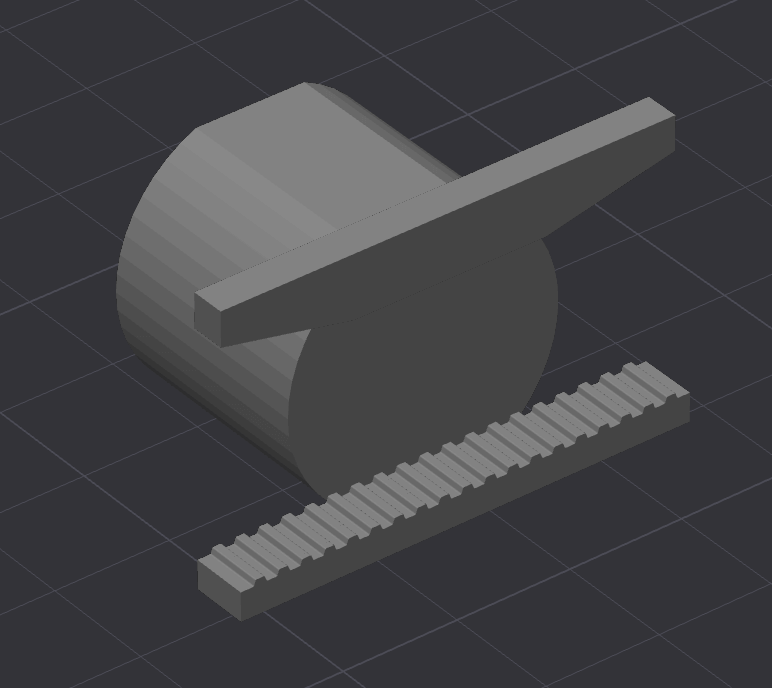
\includegraphics[width = 0.5\textwidth]{assets/figures/ameliorations/orientation_support_crémaillère.png}
    \caption{Orientation d'impression du support à crémaillère}
\end{figure}
Là aussi il conviendra de mettre des supports partout où il le faut !

\newpage
\subsection{Programme Matlab de mesure}
Comme dit précédemment, le programme pour réaliser les mesures des écrans a été réalisé sous Matlab à l'aide de la fonction "App Designer", l'interface est la suivante:
\begin{figure}[H]
    \centering
    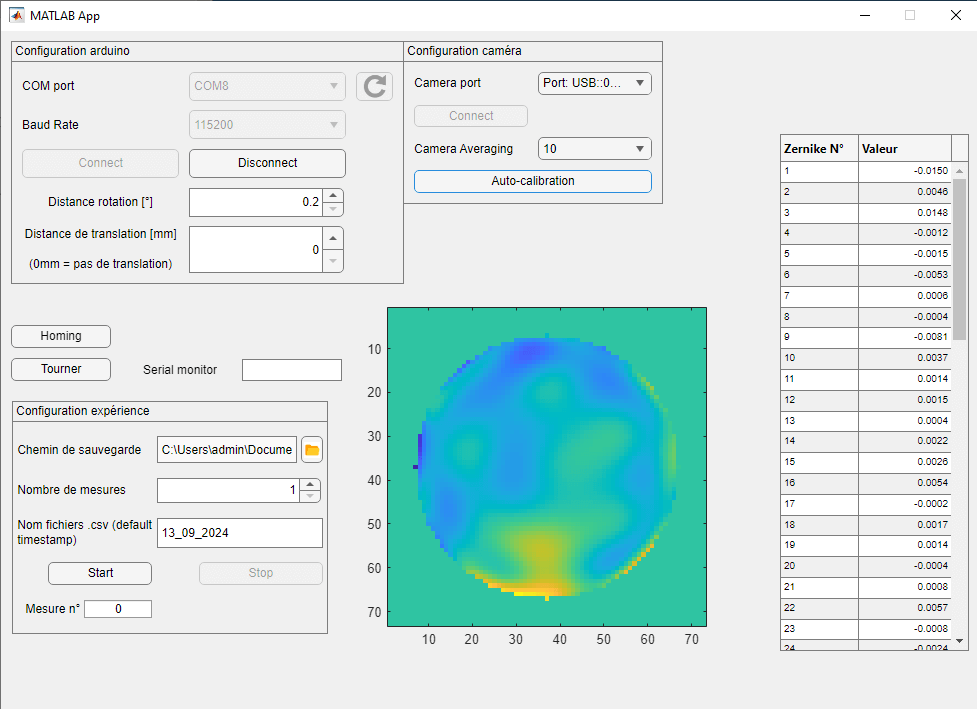
\includegraphics[width = \textwidth]{assets/figures/ameliorations/capture interface.png}
    \caption{Interface programme de mesure}
\end{figure}
Pour fonctionner, le programme a besoin de :
\begin{itemize}
    \item l'addon matlab Arduino
    \item Du programme WFS de throlabs \cite{WFS_thorlabs_site}
    \item du fichier polzer.m
    \item du fichier indzer.m
    \item du fichier polzer\_array.mat
    \item du fichier thorlabswfs.m
\end{itemize}

Le fonctionnement du programme se base sur des boutons qui déclenchent des fonctions Callbacks, donc pas de boucle principale,
ni de fonctionnement séquentiel, dans cette section il conviendra donc d'expliquer le fonctionnement et la logique derrière le processus
de mesure, pour le reste le code source est normalement suffisement bien documenté.
\newpage

\section{Fabrication des écrans}
Comme dit dans la \autoref{sec:etat de lart}, la solution sera développée autour d'une buse d'atomisation pneumatique.
Cette dernière provient du fournisseur \href{https://www.spray.com/fr-eu}{Spraying Systems Co}\footnotemark.
Le model séléctionné est le corps de buse \textbf{B1/4JN-SS} et la tête de buse \textbf{SU1-SS } qui fournira une projection en cône plein.
\begin{figure}[H]
    \centering
    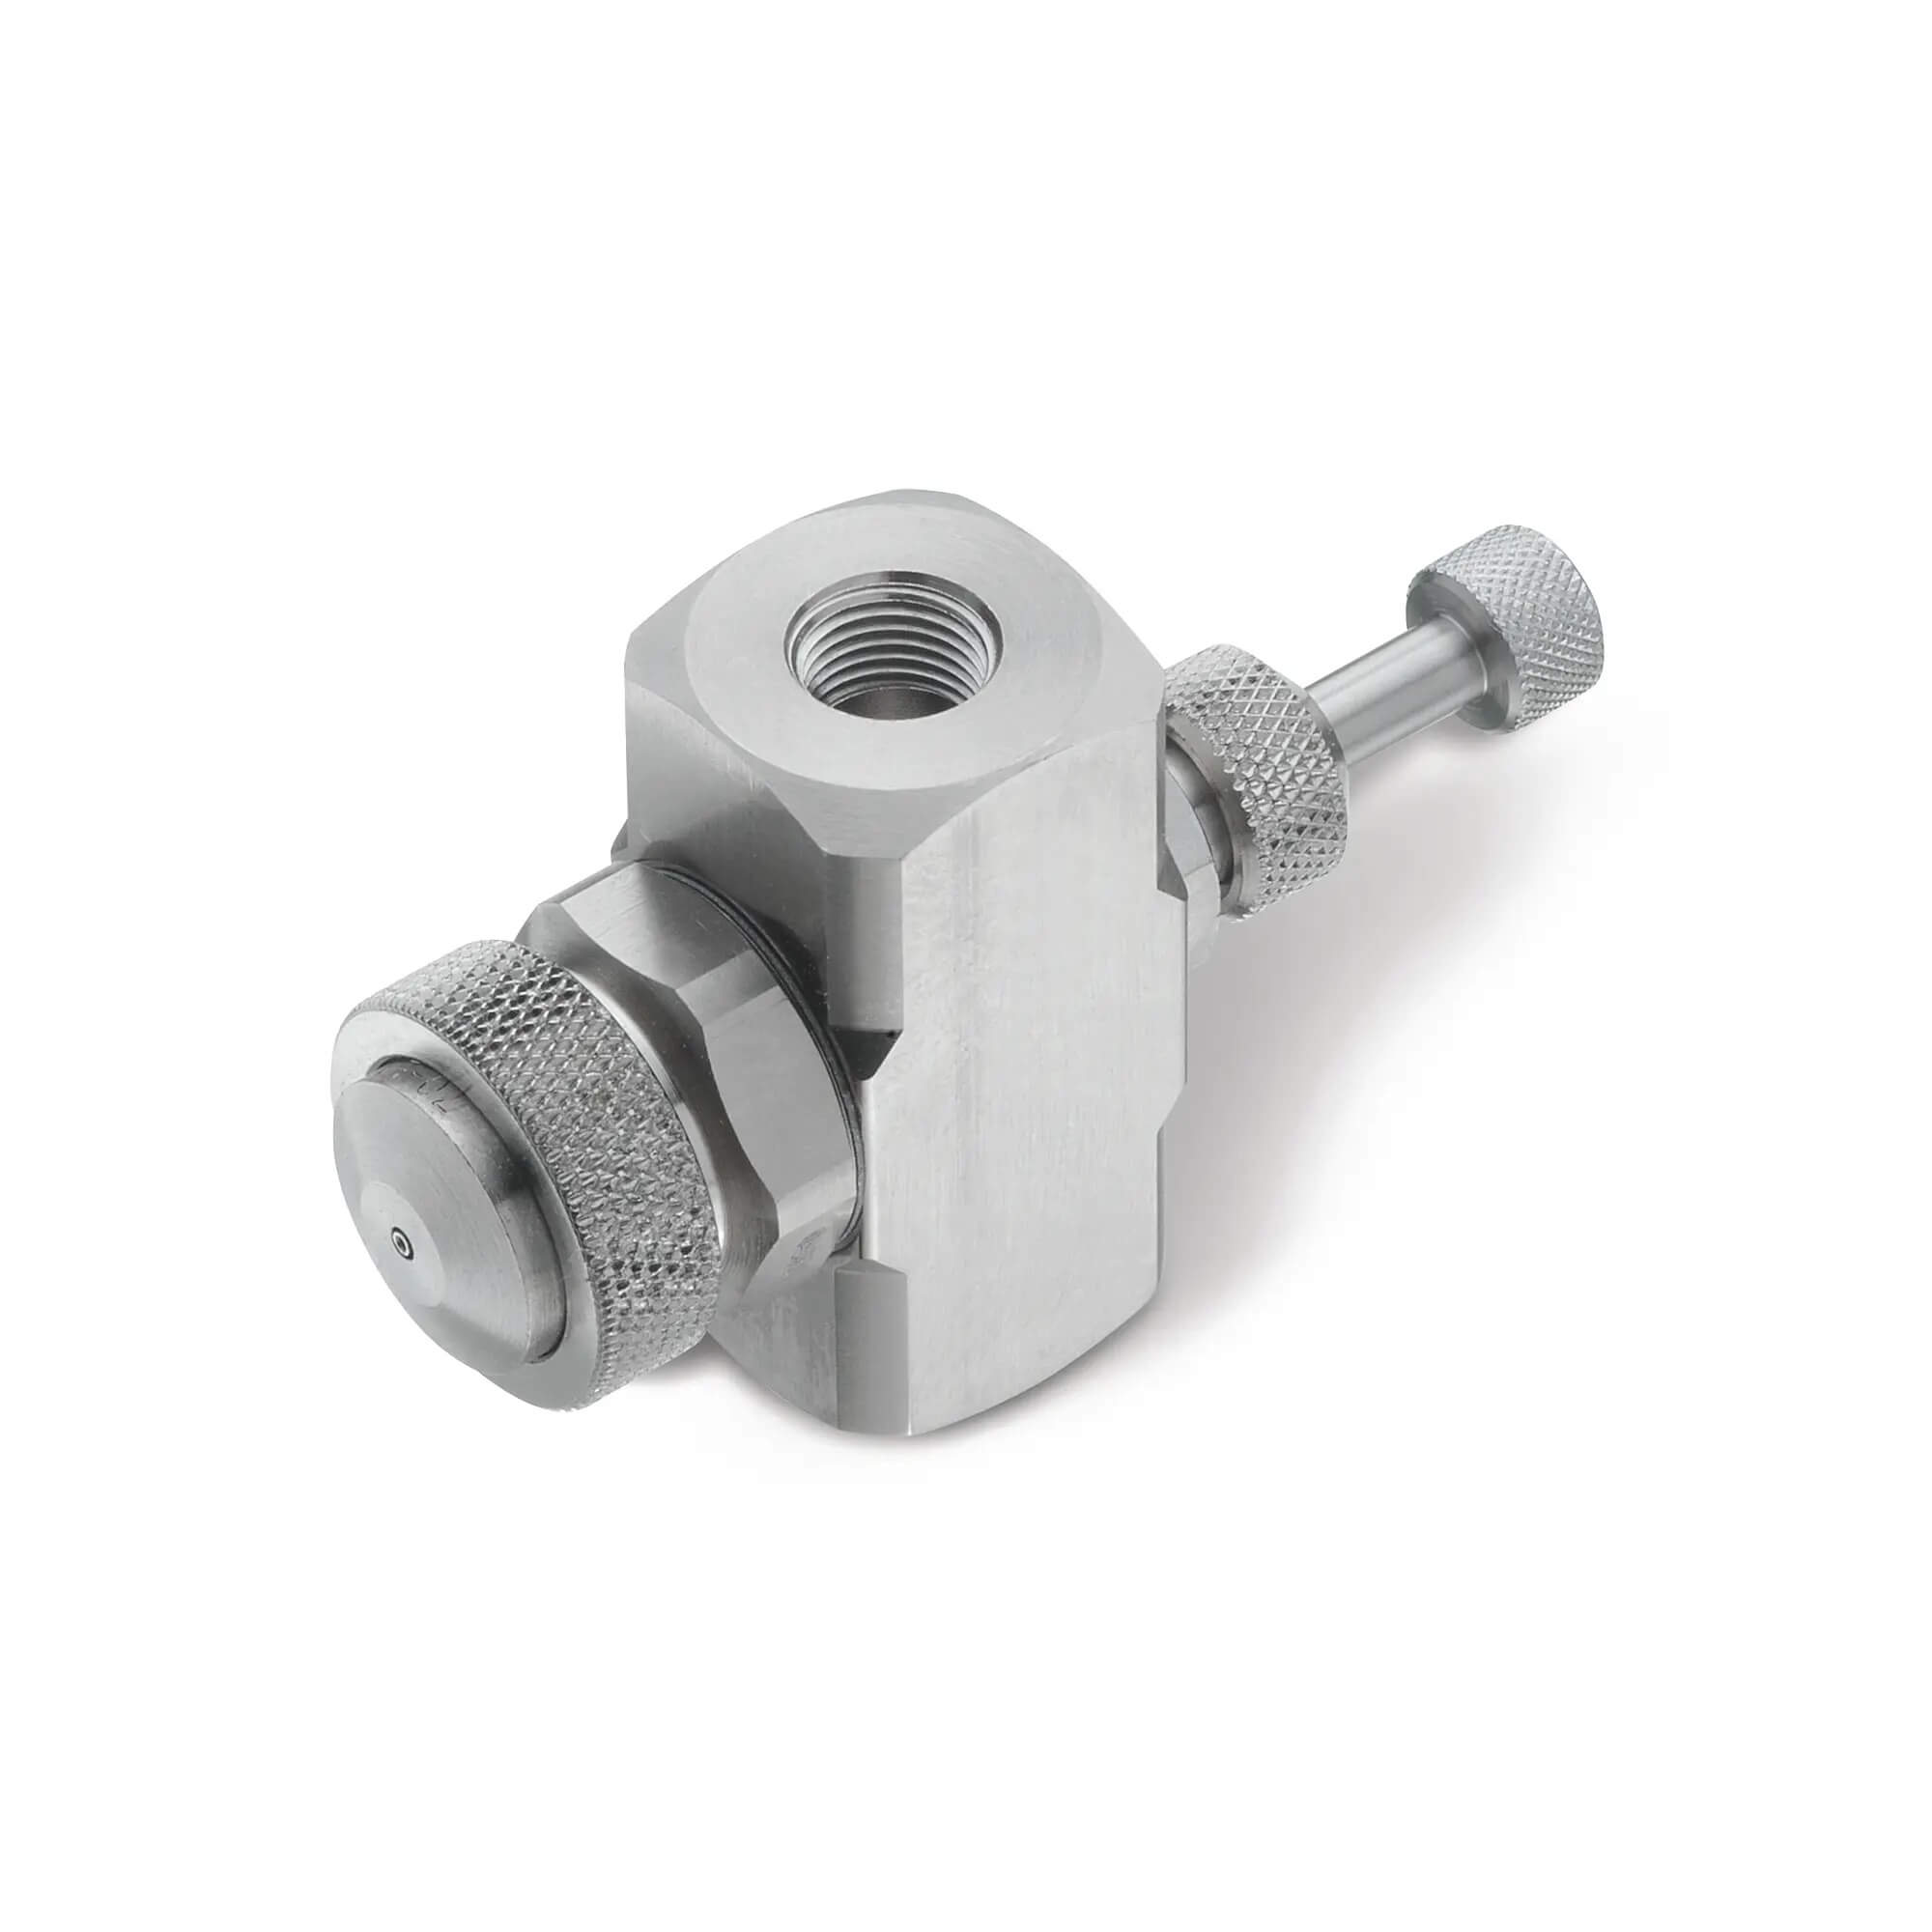
\includegraphics[width = 0.5\textwidth]{assets/figures/ameliorations/J_Series_1_8JN_and_1_4JN.jpeg}
    \caption[Buse B1/4JN-SS]{Buse B1/4JN-SS \cite{image_buse_spray_com}}
\end{figure}
Les raccords sur la le corps de la buse sont en BSPT 1/4 (donc 1/4 cônique), la buse est aussi équipée d'une aiguille de coupure manuelle du flux de liquide.
En partant donc de la machine originelle, le croquis de concept suivant a été développé:
\begin{figure}[H]
    \centering
    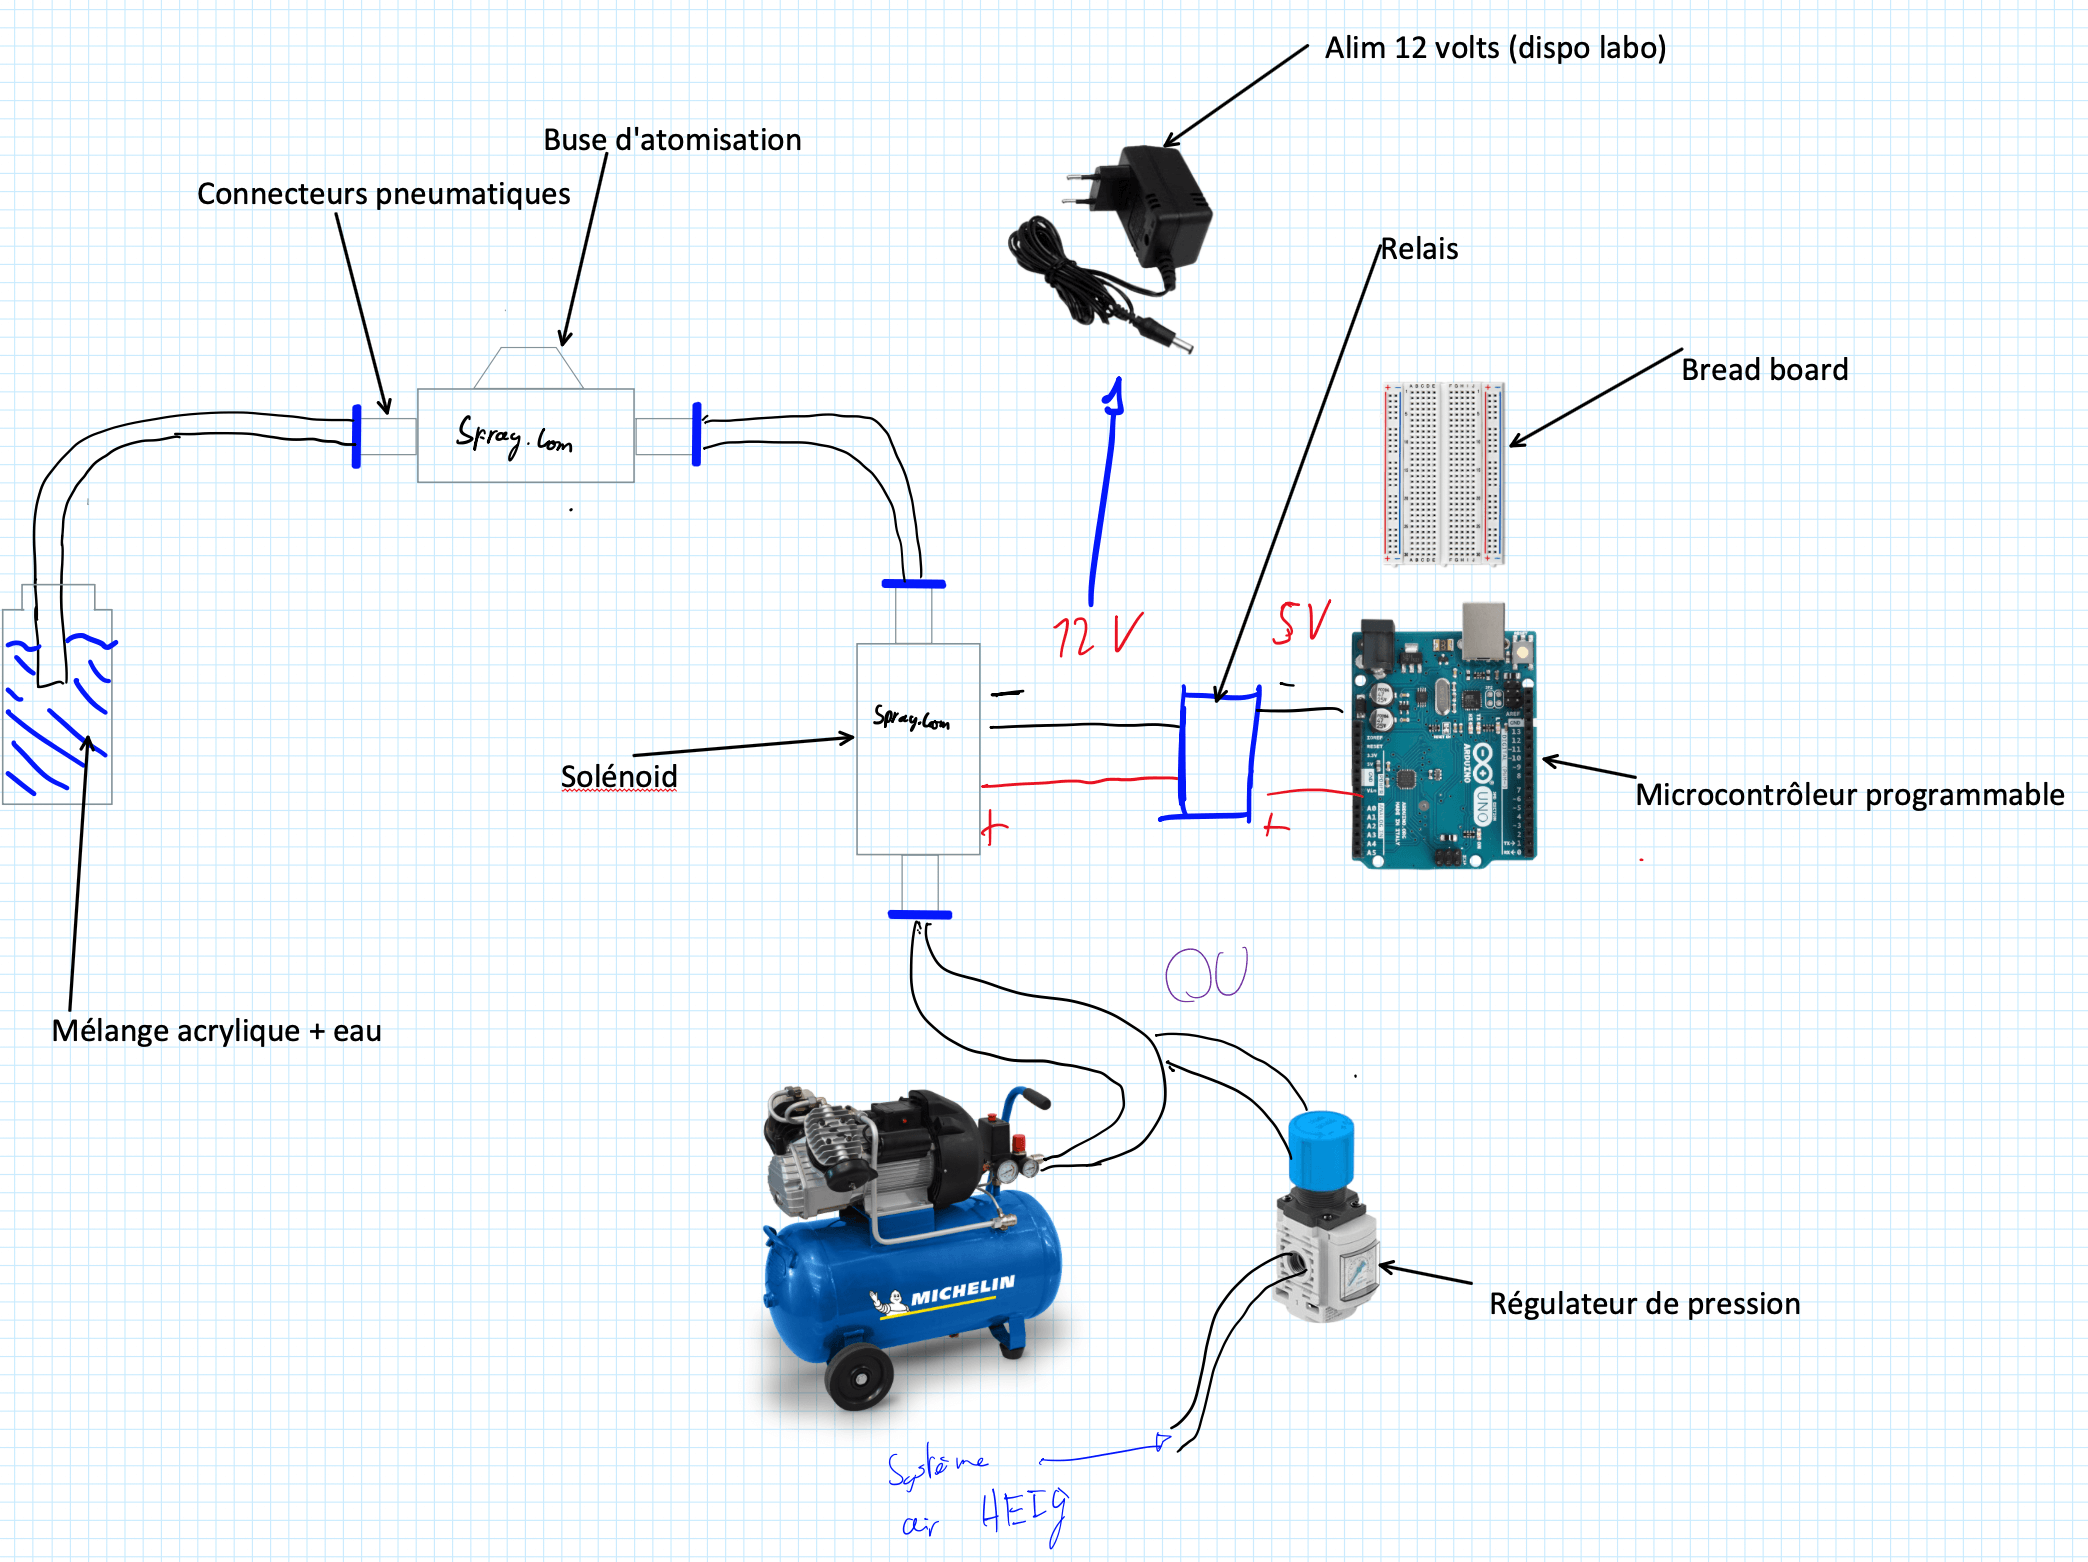
\includegraphics[width = 0.8\textwidth]{assets/figures/ameliorations/Croquis_machine_ecran_ver_1.png}
    \caption[Croquis nouvelle machine de spray ver. 1]{Croquis de la nouvelle machine de spray version 1}
\end{figure}

Cette buse est normalement capable de fonctionner uniquement avec de l'air comprimé qui créera une siphon aspirant le liquide à projeter d'une façon analogue à l'aérographe,
Malheureusement après des test préliminaires en connectant simplement la buse au système d'air de l'école et en essayant d'aspirer de l'eau, on a pu vite se rendre compte que la
configuration en siphon était problématique, en effet l'eau entrait dans la buse et était projetée une fraction de seconde avant d'être violement renvoyée dans le tuyaux d'entrée.
Il a fallu donc s'entretenir avec un conseillé de \textbf{Spraying System Co}, qui nous a donc conseillé d'utiliser une pompe péristaltique pour pousser le liquide dans la buse,
Aboutissant alors au second concept de la machine :
\begin{figure}[H]
    \centering
    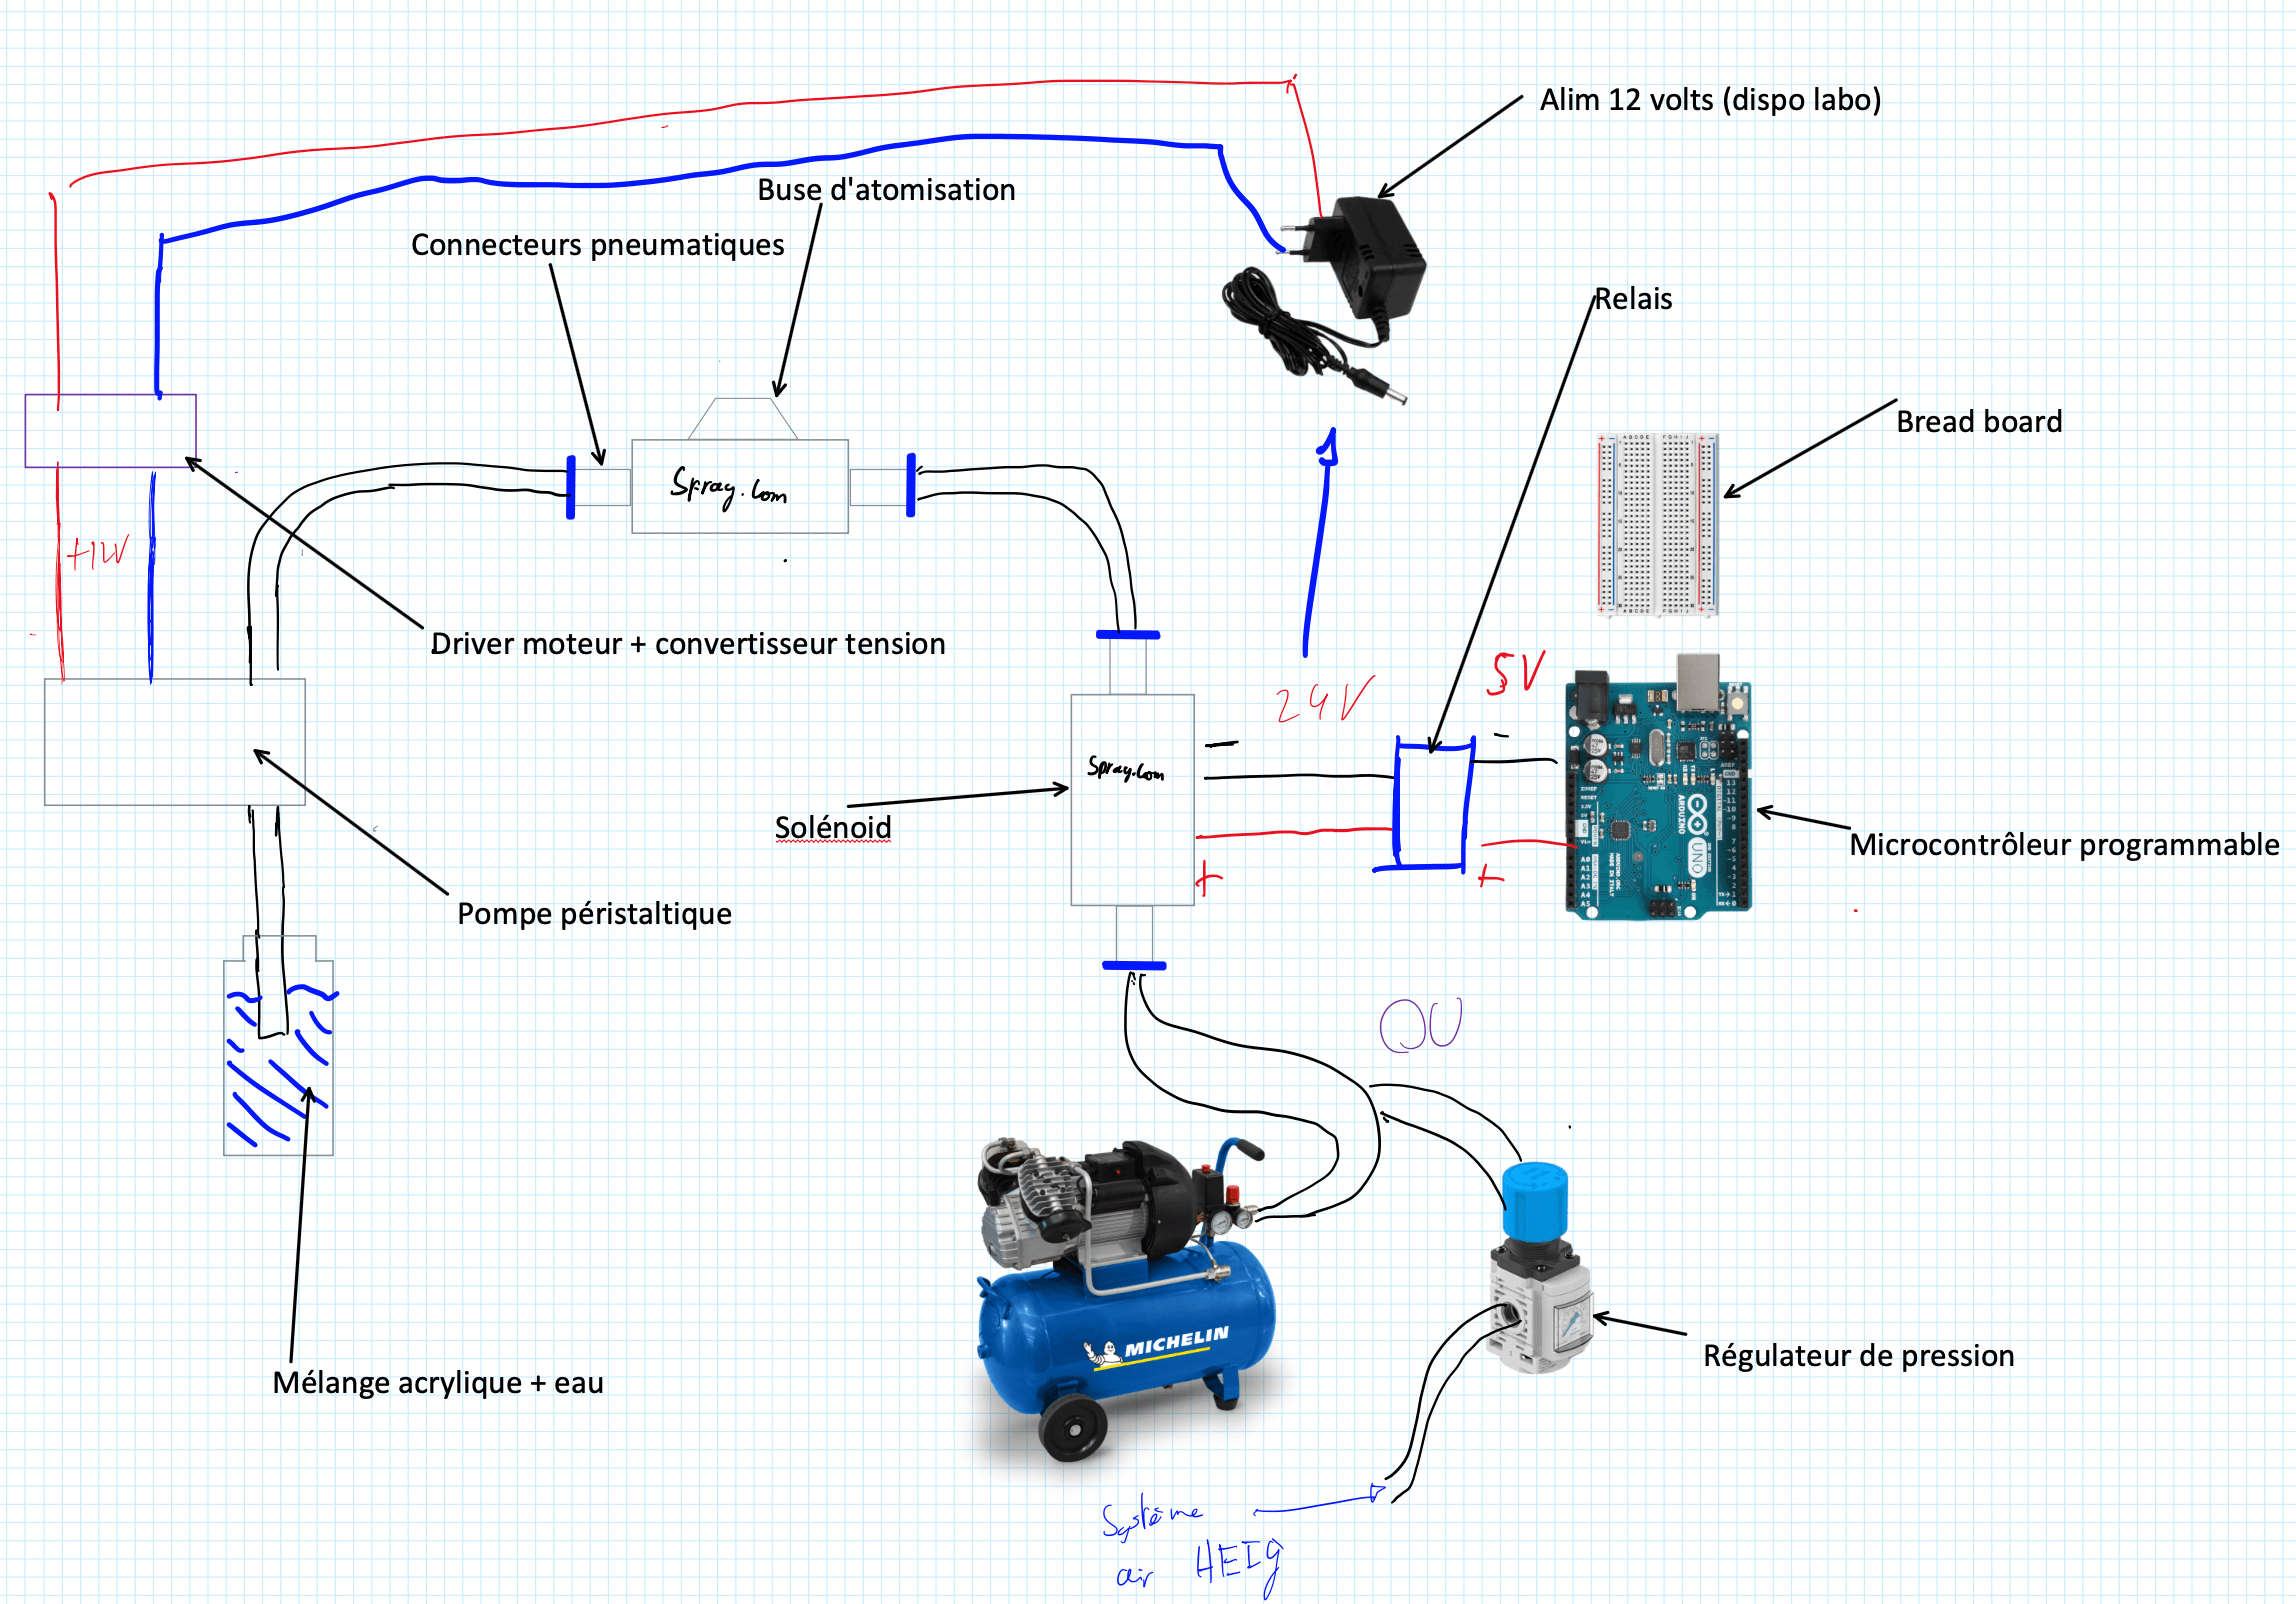
\includegraphics[width = 0.9\textwidth]{assets/figures/ameliorations/Croquis_machine_ecran_ver_2.png}
    \caption[Croquis nouvelle machine de spray ver. 2]{Croquis de la nouvelle machine de spray version 2}
\end{figure}


\footnotetext{\href{https://www.spray.com/fr-eu}{https://www.spray.com/fr-eu}}

\input{examples.tex}

\chapter{Conclusion}


\vfil
\hspace{8cm}\makeatletter\@author\makeatother\par
\hspace{8cm}\begin{minipage}{5cm}
    
\end{minipage}

\clearpage
%\bibliographystyle{plainnat}

\printbibliography

\appendix
\appendixpage
\addappheadtotoc



\let\cleardoublepage\clearpage
\backmatter

\label{glossaire}
\printnoidxglossary
\label{index}
\printindex

% Le colophon est le dernier élément d'un document qui contient des notes de l'auteur concernant la mise en page et l'édition du document : il est parfaitement optionnel.
\input{colophon.tex}

\end{document}
